\documentclass[report]{tnreport}
%\documentclass[confidential,pidr]{tnreport} % If you are writing confidential report
\usepackage{wrapfig}
\usepackage{pdfpages}
\def\reportTitle{Stage réalisé chez Déclic Communication} % Titre du mémoire
\def\reportLongTitle{Stage réalisé chez Déclic Communication} % Titre plus long du mémoire

\def\reportAuthor{Florian LAUER}
\def\reportAuthorEmail{\email{florian.lauer@telecomnancy.eu}} % Courriel de l'élève
\def\reportAuthorAddress{20, Rue des Vignes} % Adresse de l'élève
\def\reportAuthorCity{57740, LONGEVILLE-LÈS-SAINT-AVOLD} % Adresse (cont.) de l'élève
\def\reportAuthorPhone{+33 	(0)6 31 89 65 65} % Téléphone de l'élève 

\def\reportIndustrialSupervisor{Benoît BOUR} % Prénom Nom de l'encadrant industriel
\def\reportAcademicSupervisor{Isabelle HEUDIARD} % Prénom Nom de l'encadrant académique

\def\reportCompany{Déclic Communication} % Nom de l'entreprise d'accueil
\def\reportCompanyAddress{2, Avenue des alliés}  % Adresse de l'entreprise
\def\reportCompanyCity{57500, SAINT-AVOLD} % Adresse (cont.) de l'entreprise
\def\reportCompanyPhone{+33 (0)3 87 92 81 00} % Téléphone de l'entreprise
\def\reportCompanyLogoPath{figures/logo-declic} % Logo de l'entreprise -- comment this definition to remove company logo

\def\place{Nancy} % Ville pour la signature pour l'engagement anti-plagiat
\def\date{\today} % Date pour la signature de l'engagement anti-plagiat

%\def\reportProjectCustomer{Projet réalisé pour Vladimir Latocha de l'équipe EDP du laboratoire IECN}

\begin{document}

\maketitle
\pagenumbering{roman}

\insertAntiPlagiarismAgreement{LAUER, Florian}{31415656}

\cleardoublepage

\makesecondtitle

\section*{Remerciements}



\addcontentsline{toc}{chapter}{Remerciements}

{\em
Je tiens tout d'abord à remercier Monsieur Alain Letullier, co-dirigeant pour m'avoir offert la possibilité d'effectuer ce stage, pour ses conseils et son soutien tout au long de ce stage. 

Je remercie également Sébastien Albert, chef de projet, pour m'avoir confié des projets intéressants et variés pendant ce stage, ainsi que Benoît Bour, responsable informatique, pour ses conseils et sa disponibilité.

Enfin, je tenais à remercier également le restant de l'équipe de Déclic Communication, Florence, Nathalie, Yannick, Alain et Florian pour m'avoir accueilli chaleureusement au sein de l'entreprise, et pour tous les échanges d'idées intéressants que vous avons pu avoir lors des différentes réunions.
}


\section*{Avant-propos}
\addcontentsline{toc}{chapter}{Avant-propos}

Le stage de 2ème année doit permettre aux élèves-ingénieurs de découvrir et pratiquer les techniques et outils utilisés dans les métiers de l’informatique et de la production industrielle et d’être confrontés aux contraintes temporelles, économiques et humaines associées. 
Étant issu d’une classe préparatoire c’était pour ma part ma première expérience en entreprise en tant qu’informaticien, D’une durée de 6 à 10 semaines, c’est l'occasion de mettre en application certains acquis vus en cours aussi bien pour le côté technique que pour les méthodes de travail, mais aussi de se rendre compte des besoins réels en informatique en dehors du cadre scolaire.

Ce stage est également un bon moyen de faire le point sur son orientation après le diplôme, car plusieurs choix s’offrent à nous. Recherche, grandes entreprises, startups, figurent au panel de choix et ce stage a été pour moi un moyen de découvrir le monde de l’entreprise.

Tous mes collègues ont réussi dès le début à me mettre à l’aise, grâce à la réunion d’accueil habituelle organisée à l’arrivée d’un nouveau stagiaire, avec un tour de table où chacun à pu se présenter, succédé par une présentation générale de l’entreprise, des règles à respecter et des différents projets qui me seront attribués. J’ai ensuite été amené à mon poste de travail, dans une pièce appelé l’atelier, aux côtés des deux graphistes, et il a été mis à ma disposition un PowerMac G5 ainsi qu’un PC portable sous Windows 10, j’ai également reçu une adresse mail pour communiquer avec mes collègues : stagiaire@declic-communication.com.





\cleardoublepage

%\renewcommand{\baselinestretch}{0.5}\normalsize
\tableofcontents

\renewcommand{\baselinestretch}{1.0}\normalsize
\cleardoublepage

\pagenumbering{arabic}
\setcounter{page}{1}

\chapter{Introduction}
Ce rapport présente les différents travaux que j’ai effectués lors de mon stage “technicien” de deuxième année à Télécom Nancy. Mon stage a été réalisé dans la société Déclic Communication, agence de publicité à Saint-Avold. Initialement, j’ai eu la liste de sujets suivante :


\begin{itemize}
\item étude changement de logiciel CRM, récupération et fusion avec nos bases de données existantes (PHP),
\item programmation et développement informatique de projets clients,
\item projet réalisation nouvel intranet Déclic (Optimisation et évolution de l’existant),
\item analyse et optimisation SEO de sites clients,
\item optimisation SEO et performances WordPress,
\item et participation à la vie active de l’entreprise...
\end{itemize}


Par la suite il s’est avéré que ce programme subissent quelques petites modifications. Je vais donc organiser mon rapport en séparant les différents gros projets en plusieurs parties détaillées après avoir présenté l’entreprise, puis j’exposerai également les tâches plus brèves que j’ai réalisés et qui m’ont permis tout de même d’acquérir de nouvelles connaissances. Enfin, je terminerai avec un bilan du stage et de mes acquis et des quelques difficultés rencontrées.



\chapter{Présentation de l'entreprise}


Comme cité précédemment, Déclic Communication est une agence de publicité localisée à Saint-Avold, en Moselle. On peut dire que la société créée, et fabrique tous supports de communication, en passant par les solutions internet comme les sites web. L’entreprise a été fondée il y a 32 ans par M. Alain Letullier qui aujourd’hui dirige l’entreprise aux côtés de M. Sébastien Albert. Au niveau juridique c’est une SARL (Société à Responsabilité Limitée), divisée en 3 pôles que je détaillerai ensuite, et composée de 8 employés.
Ses domaines d’expertises sont :
\begin{itemize}
\item la stratégie de communication
\item la communication digitale
\item la communication et gestion événementielle
\item la communication pédagogique.
\end{itemize}


\setlength{\belowcaptionskip}{5pt}
\begin{figure}[h]
  \centering
  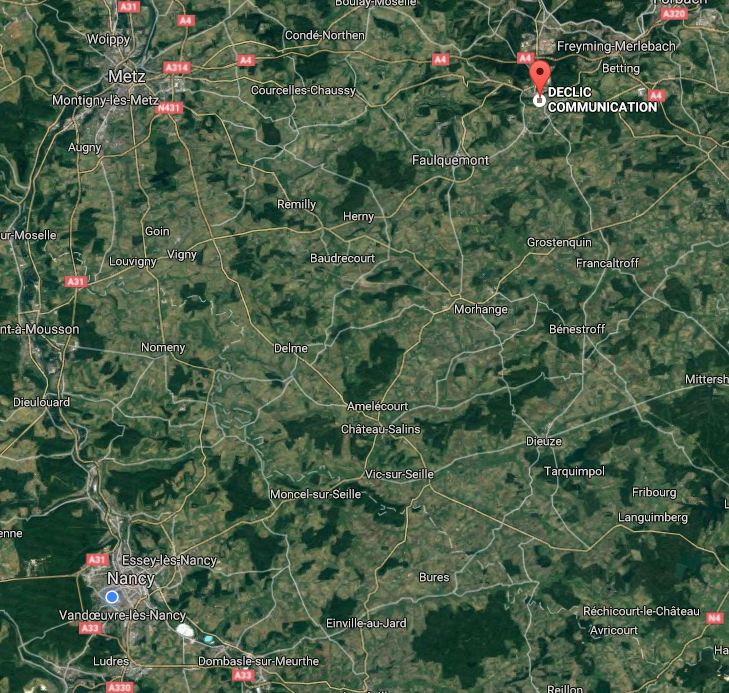
\includegraphics[width=13cm]{figures/map_plan}
  \caption{Localisation de l'entreprise en Lorraine}
  
  \label{fig:localisation}
\end{figure}
Elle fonctionne dans une logique de résultat, c’est à dire qu’il faut impérativement satisfaire le client et dans les plus brefs délais, pour continuer de s’assurer une pérennité sur le marché. Une des priorités pour l’entreprise et la sécurisation des données et la confidentialité, pour s’assurer la confiance des clients.
Les 3 différents pôles sont les suivants :
\begin{itemize}
\item conseil en création et stratégie de communication
\item fabrication, logistique et administratif
\item création, web design et solutions internet
\end{itemize}


Le pôle de conseil en création et stratégie de communication est composé des deux dirigeants ainsi que de Florian Guichon, commercial et chef de projet. C’est le pôle qui coordonnes tous les projets dans le temps, qui s’assure que les travaux soient effectués à temps et qui prospecte également de nouveaux clients.


Le pôle fabrication, logistique et administratif est composé des assistantes de production, qui gèrent par exemple les banques d’images et données informatiques, qui établissent le cahier des charges de la chaîne graphique, ou encore qui réalise le suivi commercial. Ce sont souvent elles qui sont concernées lorsqu’un client à un soucis où une requête à effectuer pour modifier un visuel.


Enfin, le pôle de création, web design et solution internet est celui dans lequel j’ai effectué mon stage. Il est composé de 3 personnes : un graphiste, un infographiste et un informaticien. Les graphistes sont ceux qui réalisent les visuels (logos, affiches, prospectus…) à l’aide des logiciels de la suite Adobe (Photoshop, Illustrator et InDesign). Ceux sont également eux qui envoient le contenu graphique des sites web que Benoît Bour, le responsable informatique, réalisent souvent grâce au CMS Wordpress.


Il faut savoir que ces pôles sont très interdépendants, en effet : lorsque qu’un client commande un nouveau produit, c’est très souvent tous les employés qui sont impliqués dans le projet. Il n’est pas rare que des gens des différents pôles réalisent des réunions.


Dans l'environnement socio-économique actuel, l’entreprise migre à l’ère du numérique, les supports papiers se font un peu moins et les sites internet nécessitent beaucoup d’entretien. Du côté de sa stratégie de développement, l’entreprise fait du prospect dans la région, elle signe également les sites qu’elle réalise ce qui améliore sa visibilité, et possède un site internet pour mettre en valeur ses compétences, en affichant certains projets qui ont déjà été réalisés. 

\begin{figure}[h]
  \centering
  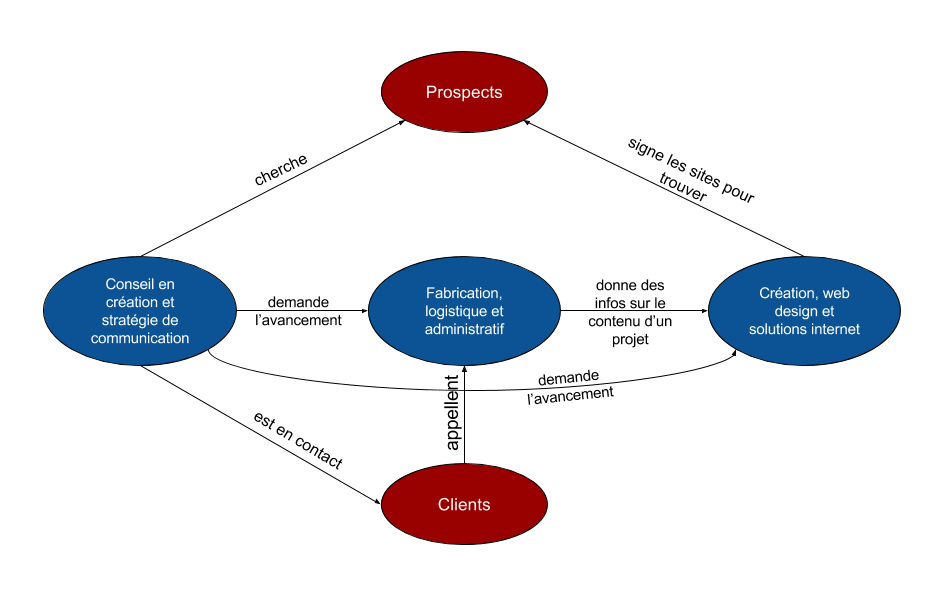
\includegraphics[width=16cm]{figures/Organigramme}
  \caption{Organigramme de travail}
  
  \label{fig:organigramme}
\end{figure}

\chapter{Processus de vérification des sites réalisés par l’entreprise}

\section{Problématique}

Il se trouve que l’entreprise possède un grand nombre de site qu’elle a réalisé et qu’elle héberge via des services externes comme OVH. Une des tâches coûteuse en temps mais qui s’avère bien pratique et la vérification de ces sites, celle ci est en général effectuée par les stagiaires lorsqu’ils arrivent dans l’entreprise. Cependant, ceux ci n’étaient pas très guidés dans leurs vérifications. On leur demande juste de vérifier les sites et de tester les formulaires présents puis d’envoyer un rapport par mail. Il m’a donc été demandé d’améliorer ce processus pour que les futurs stagiaires puissent aller plus vite pour faire un rapport plus précis sur les problèmes rencontrés.


\section{Réalisations}

Dans un premier temps il m’a donc été demandé de faire moi même la vérification manuelle des 127 sites créés par l’entreprise, car c’est la meilleure des façons de comprendre comment améliorer le processus.
Les erreurs ou problèmes que j’ai pu trouver étaient les suivants : 

\begin{itemize}
\item texte non lisible à cause d’un bouton trop petit
\item problème d’affichage des caractères spéciaux
\item envoi du formulaire de contact impossible
\item cette page n’existe pas
\item site actuellement en travaux
\item mauvaise redirection de liens
\item site non installé
\item site non hébergé
\item site en cours de réalisation
\item erreur général de SQL
\item page grise
\item site en cours d’actualisation
\item site en cours de refonte
\item erreur enregistrement contact.
\end{itemize}

Il a donc fallu prendre en compte tous ces problèmes pour améliorer le processus de test. Un des mes encadrants m’a ensuite demandé de faire des recherches pour savoir quels étaient les facteurs qui rendent un site performant, ainsi les résultats de cette recherche pourrait être incorporés dans le processus de test. Après avoir fait moi-même une analyse des informations qui se devaient être nécessaires lorsque je me rends sur un site, et des choses qui pouvaient faire en sorte que je n’y retourne plus, j’ai également effectué des recherches sur des sites internets fournissant des conseils à des entreprises pour améliorer le référencement de leur site et pour le rendre attractif. Après avoir fait le bilan des deux recherches, j’ai mis les informations en commun et les ai regroupé par thème : le fond, la forme et la technique, en séparant bien les différents moments avant, pendant et après la mise en service du site. Voir document intitulé “Les grandes étapes pour avoir un site web performant” en Annexe A.


Avec l’aide de ce document, j’ai commencé la rédaction d’un autre document qui serait donné aux futurs stagiaires lorsqu’ils arrivent, et qui les guidera durant les tests. J’ai alors séparé les tests en plusieurs parties : la technique, le fonctionnel, le contenu, et les performances. Voir document intitulé "Processus de vérification des sites" en Annexe B.
\begin{wrapfigure}{r}{6cm}
  \centering
  
\includegraphics[width=5cm]{figures/html5css3}
  \caption{Logo de HTML et CSS}
  \label{fig:logo-html-css}
\end{wrapfigure}
Ensuite il m’est assez rapidement venu à l’idée de créer une interface web sous la forme d’un formulaire permettant de réaliser ces tests facilement et également d’afficher les résultats de manière claire, avec une fonctionnalité qui attribuera une note à un site donné en fonction de sa réussite au test : mon chef de projet avait également cette idée, du coup je n’ai pas perdu de temps pour commencer un aperçu papier de ce à quoi le formulaire pouvait ressembler. 
Je l’ai ensuite fait relire par mes collègues pour qu’ils corrigent les quelques fautes et adaptent certains mots de vocabulaire au lecteur qui pouvait être en troisième par exemple.
Une fois la version papier approuvée je me suis lancé dans le développement, et il a fallu tout d’abord faire des choix techniques.
\begin{wrapfigure}{l}{6cm}
  \centering
  
\includegraphics[width=5cm]{figures/wamp}
  \caption{Logo de WAMP}
  \label{fig:logo-wamp}
\end{wrapfigure}
J’ai opté pour des technologies basiques comme HTML, CSS pour le formulaire, MySQL pour la base de donnée ainsi que Apache pour le serveur et enfin PHP pour faire des pages web dynamiques, que j’ai installé avec WAMP (Windows Apache MySQL PHP).
J’ai également opté pour ces technologiques plutôt que d’autres car elles étaient celles maîtrisées par Benoit le responsable informatique.
\begin{wrapfigure}{r}{6cm}
  \centering
  
\includegraphics[width=3cm]{figures/atom}
  \caption{Logo d'Atom}
  \label{fig:logo-html-css}
\end{wrapfigure}
Pour faciliter la tâche sur la partie CSS, j’ai utilisé le framework MaterializeCSS qui permet d’avoir une interface épurée et claire, et qui s’adapte facilement à toutes les tailles d’écran. 
Pour développer je me suis toujours servi d’Atom, qui est un éditeur de texte très performant et OpenSource.
L’interface que j’ai réalisée est en deux pages, celle du formulaire et celle d’affichage des résultats. 
A chaque envoi de formulaire, une ligne dans la base de données est créée avec les réponses fournies, et à chaque réponse un compteur de note et incrémenté plus ou moins, puis la note est rapportée sur 20. 


Les facteurs que j’ai considérés avec le plus d’importance dans l’attribution de la note ont été : affichage correct du site, de ses images, de ses textes, ancienneté de la dernière publication, pages du site vides, une page d’accueil soignée et facilement compréhensible, rang du résultat d’une recherche Google (référencement).
Sur la page rapport, c’est toujours le dernier test en date pour un site donné qui sera affiché. En cliquant sur un site dans la liste des résultats, on peut voir le détail de ses problèmes, ainsi que d’éventuels commentaires de la personne qui a fait le test.
\begin{figure}
  \centering
  
\includegraphics[width=3cm]{figures/materialize}
  \caption{Logo de Materialize}
  \label{fig:logo-materialize}
\end{figure}

Une fois l’outil terminé il a fallu le tester pour le déboguer, et je suis arrivé sur une version stable après quelques heures de débogguage.


\section{Résultats obtenus}

Une fois la version stable obtenue, il fallait procéder à l’installation pour que tous mes collègues puissent utiliser l’outil sur leur poste. Nous avons donc opté pour l’intégrer sur l’intranet sur la forme d’un lien pratique. J’ai donc déposé mes fichiers sur un serveur FTP grâce à Filezilla, mais après test sur ce serveur, j’ai rencontré une erreur de MySQL (MySQLi, que j’utilise dans mon code, n’était pas encore disponible dans la version de MySQL du serveur). Pour éviter de changer mon code, on m’a donc proposé un autre serveur, plus récent cette fois, hébergé sur un Mac. Pour le transfert de fichier je n’ai pas pu utiliser Filezilla (incompatibilité Mac) j’ai donc utilisé le Mac que l’on m’a fourni au début du stage pour transférer les fichiers via la fonctionnalité d’échange de fichiers entre Mac, la seule chose à faire pour se connecter était de rentrer l’IP de Mac sur lequel on voulait se connecter. Il a fallu que je crée le base de donnée sur le serveur MAMP (Mac Apache MySQL PHP) du Mac, et ensuite mon formulaire était accessible sur toutes les machines de l’entreprise. Dans un dernier temps il m’a été demandé de tester mon outil avec quelques sites récents réalisés par l’entreprise afin de s’assurer qu’ils auraient de bonnes notes, chose réussie vu qu’ils ont tous eu des notes supérieures à 16/20.



\chapter{Recherches dans le cadre de l’automatisation de mise à jour d’une base de données Wordpress}

\section{Problématique}
La communauté des communes de la Warndt a commandé un site internet permettant de présenter les projets, et évènements dans leurs communes, mais surtout pour répertorier les différentes entreprises et associations qu’elle possède. Le site étant déjà terminé et réalisé sur Wordpress à l’aide du thème directory, permettant d’associer à des objets de type Entreprise des adresses sur une carte Google Map. La base de données contient environ 400 entreprises et associations, toutes ont été insérées manuellement via l’interface d’administration de Wordpress, à partir de fichiers Excel les répertoriant. Le client a alors suggéré à mon entreprise qu’une solution permettant la mise à jour automatique du site (et donc de la base de données) à partir de modifications dans le fichier Excel pourrait être pratique. Or par manque de temps à y consacrer le responsable informatique n’a pas pu faire beaucoup de recherches dessus, et j’ai été affecté à cette tâche.

\section{Réalisations}

Le site étant déjà en ligne, j’ai récupérer tous les fichiers du serveur pour en faire une copie sur mon PC portable et ainsi pouvoir faire les tests sans impacter le site existant. Pour les tests j’ai utilisé l’utilitaire WAMP que j’avais déjà installé sur mon ordinateur et permettant de créer le serveur et la base de données. Il me fallait alors dans un premier temps analyser la façon dont les entreprises étaient stockées dans la base, et ce fût un gros travail car le thème Wordpress sépare les données utiles dans un très grand nombre de tables différentes. 

\begin{figure}[h]
  \centering
  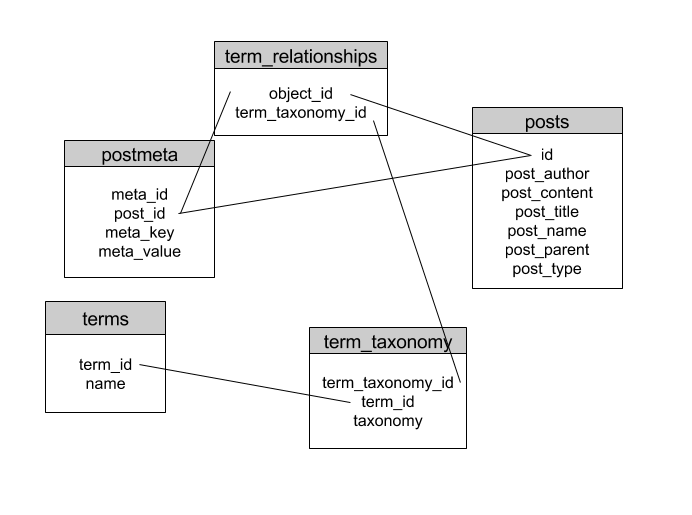
\includegraphics[width=13cm]{figures/Schema_BDD}
  \caption{Schéma des tables importantes de la base de données}
  
  \label{fig:installation}
\end{figure}


Les informations utiles affichées étaient les suivantes :
\begin{itemize}
\item Nom de l’entreprise/association 
\item Nom du contact 
\item Adresse complète
\item Type d’entreprise si c’en est une
\end{itemize}
Après avoir effectué des recherches, j’ai conclu que la meilleure des façons de dialoguer entre un fichier Excel et une base de données étaient les fichiers CSV. Ce sont des fichiers qui contiennent sur chaque ligne des caractères séparés par une virgule, correspondant aux différentes colonnes du fichier Excel.
Cependant, le type d’entreprise, l’adresse, le numéro de téléphone du contact, son mail, étaient stockés sous la forme d’une chaîne de caractère appelé tableau sérialisé que j'ai un peu réduit (voir ci-dessous).

\clearpage


\begin{lstlisting}[caption={Tableau sérialisé}, label={lst:serializedTab}]
a:29:{
s:8:"subtitle";
s:10:"IMPRIMERIE";
s:12:"featuredItem";
s:1:"0";
s:10:"headerType";
s:3:"map";
s:11:"headerImage";
s:0:"";
s:12:"headerHeight";
s:0:"";
s:3:"map";
	a:7:{
		s:7:"address";
		s:33:"5 Rue De Valence 57150 CREUTZWALD";
		s:8:"latitude";
		s:10:"49.1910937";
		s:9:"longitude";
		s:9:"6.6915101";
		s:10:"streetview";
		s:1:"0";
		s:9:"swheading";
		s:2:"90";
		s:7:"swpitch";
		s:1:"5";
		s:6:"swzoom";
		s:1:"1";
		}
s:9:"telephone";
s:10:"0613227870";
s:19:"telephoneAdditional";
s:0:"";
s:5:"email";
s:22:"gilbert.walding@ffr.fr";
s:9:"showEmail";
s:1:"1";
s:15:"contactOwnerBtn";
s:1:"0";
s:3:"web";
s:0:"";
s:12:"webLinkLabel";
s:0:"";
s:19:"displayOpeningHours";
s:1:"0";
...
s:0:"";
s:18:"openingHoursSunday";
s:0:"";
s:16:"openingHoursNote";
s:0:"";
s:14:"displayGallery";
s:1:"0";
s:7:"gallery";
s:0:"";
s:15:"displayFeatures";
s:1:"0";
s:8:"features";
s:0:"";}
\end{lstlisting}

A l’aide de la fonction serialize et de deux fichiers ci-dessous :


\begin{lstlisting}[caption={Premier CSV en entrée de mon script}, label={lst:firstEntry}]
subtitle,featuredItem,headerType,headerImage,headerHeight,map,telephone,telephoneAdditional,email,showEmail,contactOwnerBtn,web,webLinkLabel,displayOpeningHours,openingHoursMonday,openingHoursTuesday,openingHoursWednesday,openingHoursThursday,openingHoursFriday,openingHoursSaturday,openingHoursSunday,openingHoursNote,displaySocialIcons,socialIconsOpenInNewWindow,socialIcons,displayGallery,gallery,displayFeatures,features
IMPRIMERIE,0,map,,,,0613227870,,gilbert.walding@ffr.fr,1,0,,,0,,,,,,,,,0,1,,0,,0,

\end{lstlisting}

\begin{lstlisting}[caption={Deuxième CSV en entrée de mon script}, label={lst:secondEntry}]
address,latitude,longitude,streetview,swheading,swpitch,swzoom
5 Rue De Valence 57150 CREUTZWALD,49.1910937,6.6915101,0,90,5,1
\end{lstlisting}

Je suis parvenu à générer le tableau sérialisé final. L’essentiel de mon travail a été d’écrire des scripts php qui lisaient des fichiers CSV pour faire des insertions dans la base de données.

\section{Résultats obtenus}
Au final, et avec la contraite de temps d'une semaine que je me suis fixée, pour pouvoir réaliser les autres tâches j'ai uniquement réussi à remplir les tables posts et post\_meta, il me manquait encore 3 autres tables minimum pour terminer le travail. Mon chef de projet a donc informé au client qu’il aurait fallu beaucoup plus de temps et quelqu’un de très expérimenté en SQL pour réaliser cette tâche en entier.

\chapter{Le projet du château de Saint Sixte}

\section{Problématique}
Un châtelain possédant un château à Freistroff réalisait souvent des visites de son château pour des classes des différentes écoles de Moselle, et il a décidé de rendre ses visites plus interactives en ajoutant une touche de numérique. En effet, il souhaitait que ses visiteurs puissent se connecter sur un réseau wifi non connecté à internet dans le domaine du château afin d’accéder à un site décrivant les différents lieux cultes du château. Il souhaitait également intégrer un quizz sur ce site mobile avec des questions relatives à la visite. Mon collègue informaticien à donc réalisé un site Wordpress responsive suivant ce cahier des charges, et acheté le matériel nécessaire à l’installation dans le château (Mac pour héberger le site, routeur et antenne wifi longue portée). Le site doit être disponible en français, allemand, et anglais.

\section{Réalisations}

Une de mes premières tâches pour ce projet a été l’ajout d’un bouton page précédente sur chaque page du site à la demande du client. Ensuite, j’ai ajouté les pages relatives aux langues étrangères car celle ci n’étaient pas encore créées. C’est le client lui même qui se chargerait des traductions du contenu. Lors de cette tâche j’ai du éditer des liens qui n’étaient plus adaptés lors de l’ajout des pages allemandes et anglaises (ajout de /en/ ou /de/). Ensuite j’ai fait en sorte que le serveur MAMP installé sur le Mac se lance automatiquement au démarrage grâce à un petit script en AppleScript pour gagner en efficacité et éviter au client de le faire à chaque fois.


Une fois le contenu et les pages terminés, il a fallu commencer les tests de connexion au réseau local du Mac avec des téléphones mobiles.


\begin{figure}[h]
  \centering
  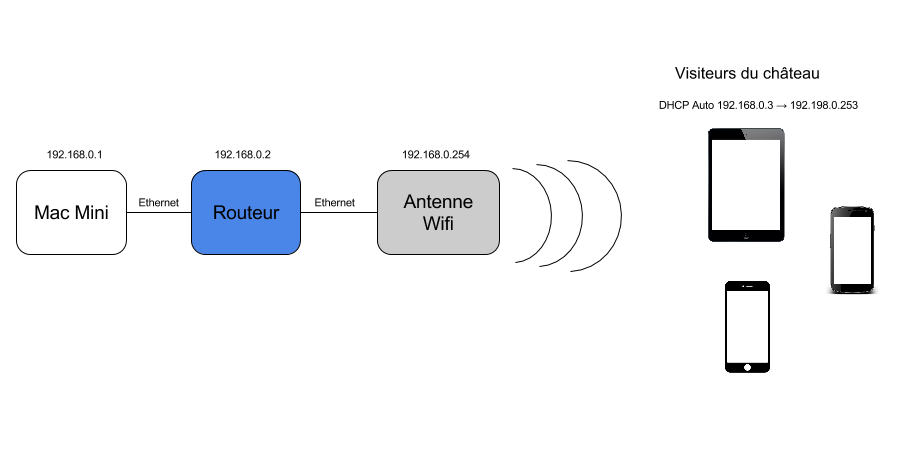
\includegraphics[width=18cm]{figures/Montage}
  \caption{Schéma de l'installation}
  
  \label{fig:installation}
\end{figure}


Alors que mes collègues possédant des iPhone ne possédaient aucun problèmes pour se connecter au localhost (à l’adresse IP) du Mac hébergeant le site web, mon téléphone Android ainsi que tous les autres sur cet OS n’y parvenaient pas. Il s'ensuit alors une longue série de tests, de changement de paramètres de configuration du routeur, de l’antenne, mais en vain. Il était impossible de se connecter à un réseau wifi ne possédant pas internet avec un téléphone Android. J’ai donc fait des recherches et trouvé des articles récents expliquant que c’était dû à une mise à jour après la version 5 d’Android : en effet, quand le réseau wifi n’a pas d’accès internet, le téléphone va tenter de se connecter avec le réseau mobile (4G) ce qui est impossible pour atteindre une IP locale. (Voir Webographie)

J’ai également fait des analyses de paquets avec Wireshark car mon téléphone avait bien une IP qui lui était affectée, et en filtrant les échanges avec uniquement mon IP je me suis aperçu que les seuls échanges avec le routeur étaient des protocoles IGMPv2 (Internet Group Management Protocol) et MDNS (Multicast Domain Name System) mais après avoir analysé plus en détail le contenu de ces paquets il s’est avéré qu’il s’agissait uniquement des tentatives de connexion au PlayStore dans le but des vérifications des mise à jour des applications. J’ai posé mon problème sur le site StackoverFlow et l’unique solution que j’ai reçue était d’utiliser l’outil Ngrok. C’est un petit script qui réalise un tunnel à partir d’internet vers le port de mon choix sur ma machine locale. Plus concrètement, il permet de partager son localhost à des utilisateurs lambdas via un URL généré automatiquement et hébergé en ligne. Or, à chaque fois que le script est lancé, l’URL est différent, de plus, le but était d’être indépendant d'internet. 


Après avoir passé plusieurs jours dans les recherches et sans obtenir de réponses, mon chef de projet a proposé de ramener le matériel à un employé de l’entreprise qui avait vendu l’antenne wifi, spécialiste du réseau. Après quelques jours, j’ai récupéré le matériel et appris qu’il avait configuré un serveur DNS sur une machine virtuelle Debian. (Voir Webographie)


Il m’a expliqué qu’il suffisait de lancer la machine virtuelle pour que tout fonctionne. Or, cela n’a pas fonctionné directement, j’ai donc utilisé Teamviewer couplé au téléphone pour tenter de régler le soucis. Il s’est avéré qu’il avait oublié de supprimer des anciens fichiers après ses premiers tests qui étaient en conflit avec la configuration actuelle.


Une fois ce problème résolu, j’ai testé la connexion avec mon téléphone Android, mais cela fonctionnait uniquement avec un port Ethernet du routeur connecté à internet. En rappelant l’expert en réseau, je l’ai informé sur les recherches que j’ai faites et il n’a pas été étonné par mes trouvailles. Je l’ai donc expliqué à mon chef de projet, et après concertation nous avons dû imposer une connexion internet au client pour un fonctionnement correct de l’installation.


Enfin, quelques jours plus tard, je suis allé au château avec mon collègue pour installer tout le matériel, nous avons pu nous connecter à une livebox. Après un problème de conflit d’IP (les IP du Mac, routeur et de l’antenne étant manuelles et initialement prévues en 192.168.1.1 pour un fonctionnement hors ligne) nous avons changé rapidement l’IP de la livebox, et pu faire fonctionner le site internet sur tous les types de mobile se connectant à l’antenne wifi.


\section{Résultats obtenus}
C’était le projet auquel j’ai participé pendant le plus de temps, le fil conducteur de mon stage et j’ai pu participer au dénouement de celui ci peu avant la fin de mon stage, ce qui m’a vraiment soulagé après les déboirs et incompréhensions que j’ai rencontrés lors de mes recherches et tests. Il m’a permis de me rendre compte des contraintes techniques qu’il fallait parfois imposer à un client, et des imprévus que l’on peut rencontrer lorsqu’on fait une installation en réseau local, en effet mes collègues n’avaient pas pensé passer autant de temps sur ce projet. Cela a été aussi un bon moyen pratique d’améliorer mes connaissances en réseau.

\chapter{Etude dans le but d’une éventuelle migration de logiciel CRM}

\section{Problématique}

Mon entreprise possède un logiciel CRM (Costumer Relationship Management) appelé Logipub depuis maintenant plus de 20 ans, cependant, aucune mise à jour n’a été effectuée depuis une bonne dizaine d’années, et l’entreprise qui vend le logiciel n’est plus très à l’écoute de ses clients aujourd’hui. Par conséquent, il m’a été demandé de faire une étude des logiciels CRM existants, et plus précisément ceux gratuits et opensource. Le logiciel CRM permet à l’entreprise :
\begin{itemize}
\item la gestion des dossiers
\item la gestion des flux clients (devis, bons de livraison, factures)
\item la gestion des flux fournisseurs (demandes de prix, bons de commande, factures d’achat)
\item la gestion des flux internes (frais, temps passés sur un projet)
\item d’avoir un tableau de bord
\item le transfert en comptabilité
\item d’avoir un planning de production
\item d’avoir un intranet
\item d’avoir un agenda.
\end{itemize}
Ce logiciel tourne en version serveur un PC et les Mac de mes collègues possèdent des licences clients.


\section{Réalisations}
\subsection{Récupération des données}
Un des premiers problèmes a été la récupération des données existantes (factures, contacts, devis, bons de livraison…) sur la base de données actuelles. C’est une base de données 4D, technologie apparue il y a plus de 25 ans, et qui aujourd’hui a une bien plus petite communauté de développeurs que SQL par exemple. Mon collègue Benoît m’a donc fourni tous les fichiers en sa possession sur le serveur contenant les données importantes. Lors de mes premières recherches assez générales, je me suis aperçu que très peu de forum relataient ce genre de récupération, ou alors les topics dataient d’il y a plus de 7 ans.
Ensuite, je me suis intéressé aux fichiers que j’avais en ma possession : les extensions étaient .4DD .4DR .4DS ; or voici les informations que j’ai trouvées sur internet :
\begin{itemize}
\item 4DB = c'est le "source" du développement, à conserver précieusement (structure de la base de données, écrans, code…)
\item 4DC = source compilée, il n'y a rien à en faire car le source n'est plus accessible, sert juste au déploiement
\item 4DD = données, tout le travail de saisie des utilisateurs, à garder 
\item 4DR = ressources du 4DD, aucun intérêt
\end{itemize}
J’avais donc bien un fichier de données, mais pas le fichier source qui permet d’avoir la structure de la base de données. J’ai donc relayé l’information à mon collègue en lui suggérant qu’il était peut être en la possession de la société qui leur a vendu le logiciel.


\subsection{Comparatif des solutions actuelles de logiciels CRM}

Ensuite, j’ai créé le tableau ci-dessous qui récapitule et compare les recherches que j’ai faites sur internet au sujet des logiciels gratuits existants. Il faut savoir que les certains ERP (Enterprise Resource Planning) sont liés aux CRM dans quelques cas : l’unique différence est qu’un CRM est orienté clients et propects, tandis que les ERP sont orientés gestion centralisée entre les différents départements de l’entreprise, mais les deux types de logiciels peuvent avoir des fonctionnalités en commun. (Voir tableaux en Annexe C)


\subsection{Installation et tests du logiciel Dolibarr}

Lors de ma première réunion à ce sujet avec Sébastien le chef de projet, il m’avait parlé de Dolibarr, qui est un CRM gratuit et opensource. Après mon étude comparative, nous en sommes venus à la conclusion que c’était celui le plus complet, il m’a donc proposé de le tester sur mon Mac.


J’ai donc téléchargé un installateur qui fonctionne comme MAMP, car cet ERP est composé d’un serveur Apache et d’une base de données MySQL. Après configuration de la base de données, et du logiciel, auquel on accède via son localhost, j’ai commencé à prendre en main le logiciel (customisation de l’apparence du logiciel, création de clients, de factures, devis… Voir Annexe D). J’ai ensuite mis du temps à comprendre comment mettre à jour le logiciel ; le Mac étant assez ancien, l’installateur n’était disponible que dans une ancienne version. Il fallait extraire la version suivante de la version installée dans le fichier htdocs de Dolimamp (équivalent de MAMP dont j’ai parlé précédemment) en prenant soin de retirer le fichier install.lock chargé de bloquer les mises à jour inopinées par des utilisateurs ayant accès au dossier puis se reconnecter à son localhost pour avoir accès à la page de mise à jour. J’ai donc fait plusieurs mises à jour successives de la version 3.1 à 3.5 (une par une, 3.1 → 3.2 etc...). Il s’est avéré que la version 3.5 était la dernière compatible avec ma version de PHP, et que cette version de PHP était la dernière compatible avec mon Mac, je me suis donc arrêté à la 3.5.


\subsection{Comparatif entre Logipub et Dolibarr}

Une fois le logiciel Dolibarr testé, on m’a fait essayé le logiciel Logipub que mes collègues utilisaient. Ensuite, on m’a demandé de réaliser un comparatif des fonctionnalités entre Logipub et Dolibarr, que vous pouvez voir sur ce tableau :
\begin{figure}[h]
  \centering
  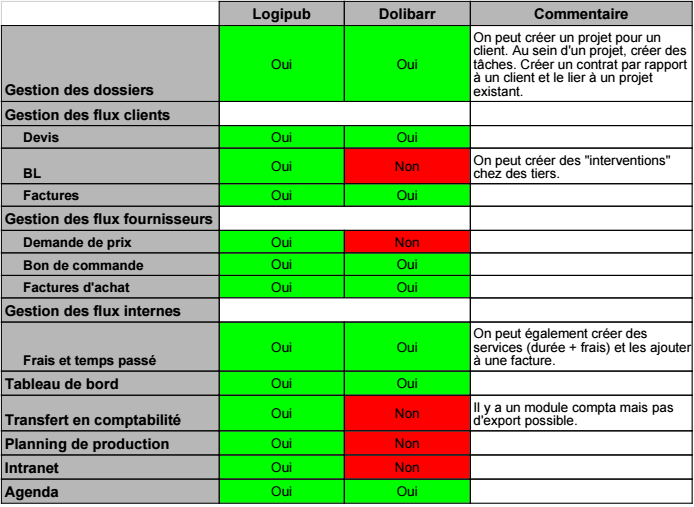
\includegraphics[width=13cm]{figures/dolibarrVSlogipub}
  \caption{Comparatif Logipub/Dolibarr}
  
  \label{fig:comparatif}
\end{figure}


\subsection{Que se passera t’il dans le cas d’un crash du logiciel Logipub ou d’un serveur ?}

Alain, un des dirigeants m’a demandé de rédiger un rapport pour savoir ce qu’il se passerait si le logiciel Logipub ou son serveur crashait. Je suis donc allé demander des informations à mon collègue responsable de l’informatique pour obtenir davantage de précisions sur l’installation. J’ai donc appris que le serveur Xserve qui sert actuellement à l’échange des données lors des projets était équipé de la technologie RAID 1 (Redundant Array of Independent Disks) qui consiste à utiliser 2 disques durs sur les 4 existants afin d’avoir une copie permanente de ce qui est effectué, cela permet d’assurer la sécurité des données en cas de dégradation d’un disque.


Par contre, il a été convenu avec mon collègue informaticien que si le logiciel Logipub venait à crasher, plus rien ne pouvait fonctionner. C’est pourquoi j’ai donc conseillé d’essayer de contacter encore et encore l’entreprise qui a vendu ce logiciel pour le mettre à jour sur un serveur plus récent équipé de cette technologie RAID avec une version plus récente du logiciel. J’ai également cité les meilleures façons d’anticiper un tel problème, il faut :
\begin{itemize}
\item faire des sauvegardes
\item faire de la maintenance régulière
\item avoir du matériel de remplacement
\end{itemize}
afin d’éviter :
\begin{itemize}
\item une perte de rentabilité
\item une perte de clients
\item une perte d’argent.
\end{itemize}

\section{Résultats obtenus}

Après avoir faits ces multiples recherches, j’ai réalisé un mail bilan avec les solutions que je pouvais proposer que voici :

\begin{itemize}
\item Contacter Open Mac pour leur demander s’ils peuvent fournir le fichier structure. Cela ne résoudra pas le problème d’export et de sécurisation, il sera sûrement alors uniquement possible de “visionner” la base de données. Le mieux étant de leur demander s’ils ont déjà effectué une telle migration (vers base de données MySQL) par le passé, car aucune recherche Google spécifique à “migration base de données logipub” n’aboutit. Par contre une mise à jour de Logipub ne résoudra pas ce problème d’export.
\item Contacter 4D pour leur poser le problème, avec les outils que nous possédons et vers où nous voudrions nous diriger.
\item Opter pour une mise à jour de Logipub en essayant (encore) de contacter Open Mac et ne pas s’orienter vers Dolibarr.
\item Entrer les données à la main sur Dolibarr me paraît être une tâche incommensurable. Pour faire une automatisation de cette tâche il faudrait auparavant résoudre les problèmes d’export de l’ancienne base de données cités précédemment.
\end{itemize}

\chapter{Développement d’un email responsive design}

\section{Problématique}
Une des activités de l’entreprise est de réaliser des campagnes d’emailing de publicité, c’est à dire qu’ils envoient grâce à un logiciel qu’il lit une base de données d’adresses email une grosse quantité d’emails pour des clients. Lors de mon stage, un des clients a demandé s’il était possible d’avoir un mail qui serait responsive c’est à dire où il n’y aurait pas besoin de zoomer lorsqu’on est sur un smartphone et qui s'adapterait à l’écran. C’est quelque chose qui n’avait jamais été fait auparavant par mes collègues, je me suis donc proposé de faire un essai et de leur montrer ce qui était faisable.

\section{Réalisations}

Il faut savoir qu’une publicité par email est tout simplement une page HTML accompagnée de propriétés CSS.
J’ai donc téléchargé un template gratuit de mail responsive pour voir comment cela fonctionnait. L’astuce principale est d’utiliser des emboîtements de tableaux pour que si la page sur laquelle on affiche le mail est trop petite, le tableau qui est a droite passe en dessous.
On m’a donc fourni un premier mail en format HTML assez simple pour me faire la main et j’ai réussi à faire en sorte qu’il soit responsive.
Ensuite, on m’a donné le fichier Photoshop du mail du client qui aurait souhaité avoir une version responsive car il n’y avait pas encore de version HTML, ainsi que tous les visuels et la charte graphique (polices, couleurs). J’ai donc fait en sorte de reproduire dans le moindre détail cette image issue de Photoshop sur ma version HTML, que j’ai adaptée pour que ce soit responsive. Une autre astuce de celle des tableaux sont les medias queries (voir exemple ci-dessous) : ils permettent de définir des propriétés CSS pour une certaines largeurs d’écran. La plupart du temps je m’en suis servi pour qu’une div HTML prenne la largeur entière de l’écran une fois que la taille de l’écran est inférieure à la largeur du mail. 

\newpage
\begin{lstlisting}[language=html, caption={Exemple de media queries}, label={lst:mediaQuery}]

@media only screen and (max-width: 840px) {

	div[class="column"] {
		 width: auto!important; 
		 float:none!important;
		 padding-left: 20px!important;
	 	 padding-right: 20px!important;
		 padding-bottom: 0px!important;
	 }
	  
	 table[class="responsive"]{
		 padding-bottom: 15px!important;
	 }
}

\end{lstlisting}

\section{Résultats obtenus}

On peut voir les résultats que j’ai obtenus ci-dessous : 

\begin{figure}[h]
  \centering
  
\includegraphics[width=13cm]{figures/aje1}
  \caption{Version PC : première partie}
  \label{fig:aje1}
\end{figure}

\begin{figure}[h]
  \centering
  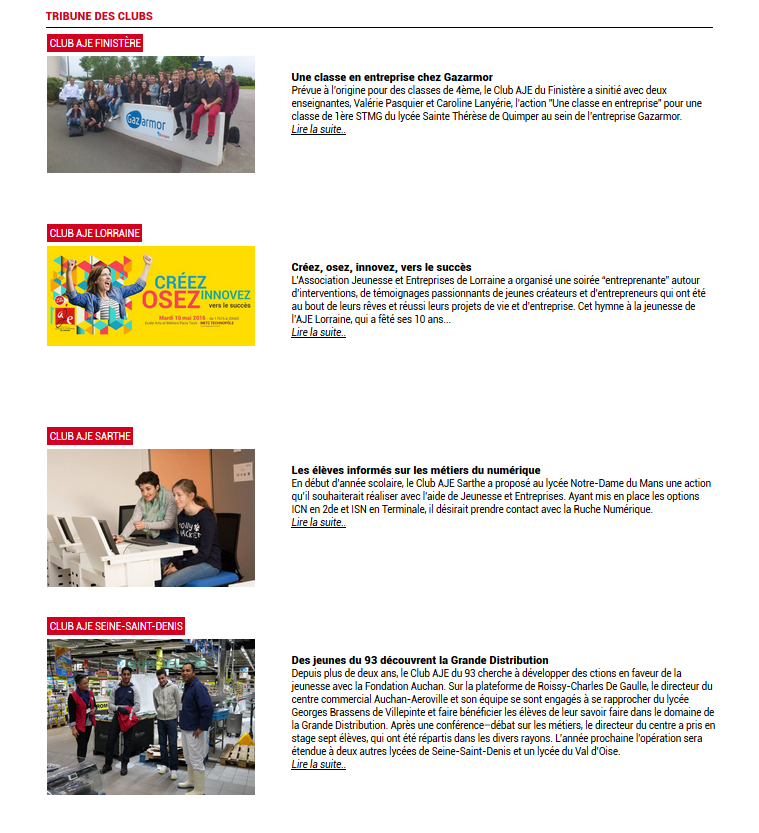
\includegraphics[width=13cm]{figures/aje2}
  \caption{Version PC : deuxième partie}
  \label{fig:aje2}
\end{figure}

\begin{figure}[h]
  \centering
  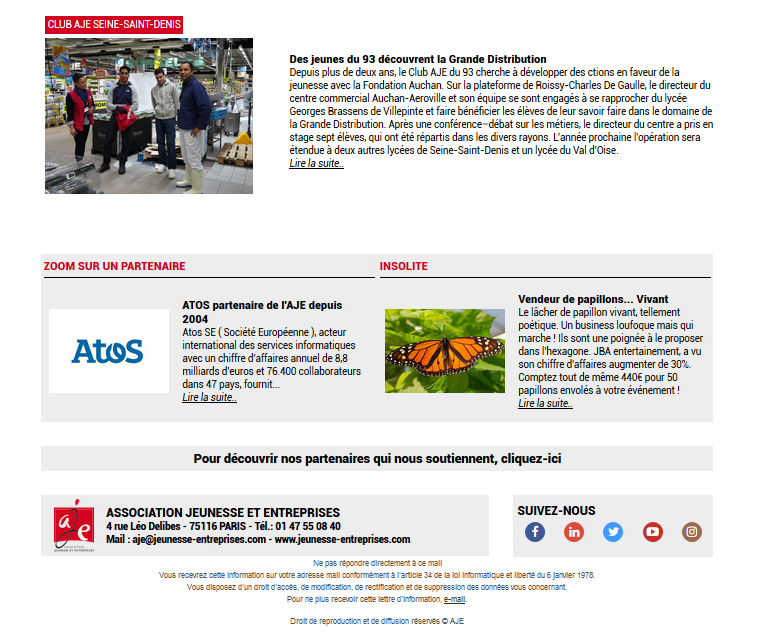
\includegraphics[width=13cm]{figures/aje3}
  \caption{Version PC : troisième partie}
  \label{fig:aje3}
\end{figure}

\begin{figure}[!htb]
\minipage{0.32\textwidth}
  
\includegraphics[width=\linewidth]{figures/aje_mobile1}
  \caption{Version mobile : première partie}\label{fig:aje_mobile1}
\endminipage\hfill
\minipage{0.32\textwidth}
  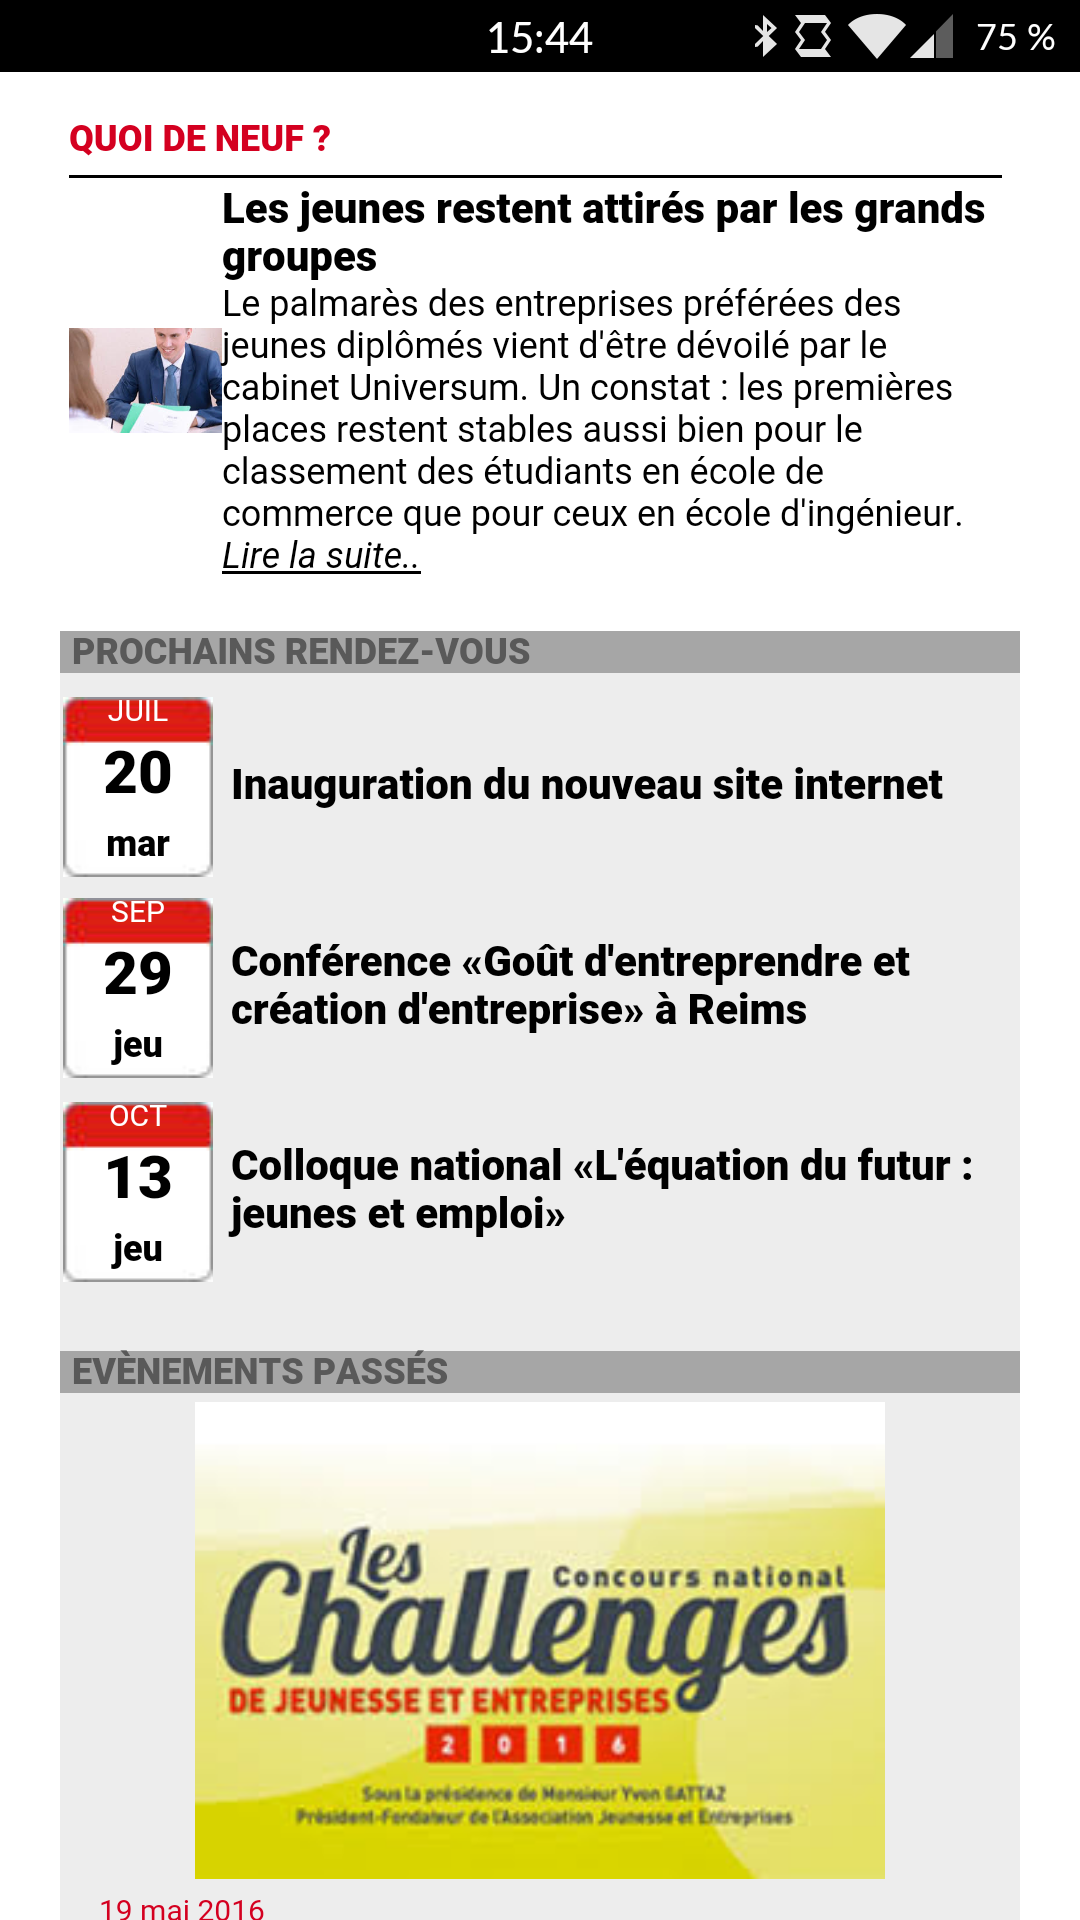
\includegraphics[width=\linewidth]{figures/aje_mobile2}
  \caption{Version mobile : deuxième partie}\label{fig:aje_mobile2}
\endminipage\hfill
\minipage{0.32\textwidth}%
  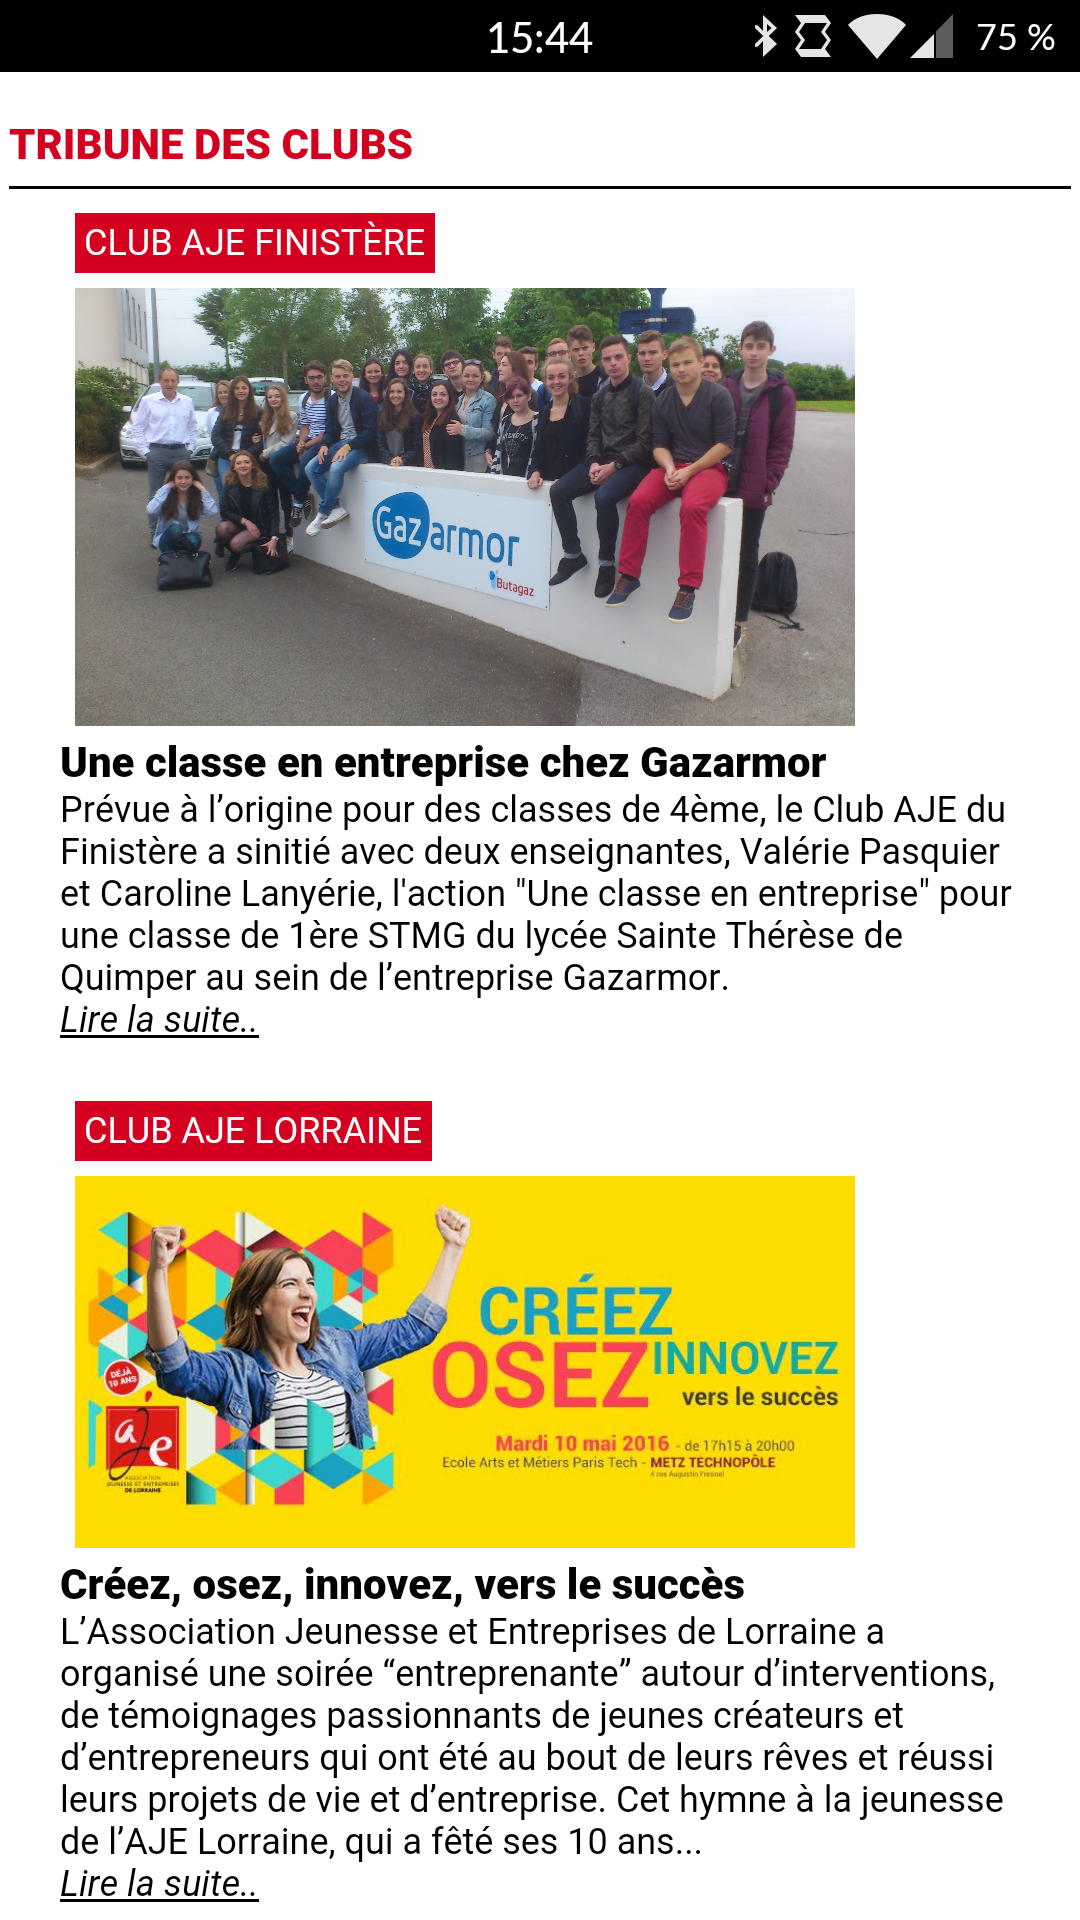
\includegraphics[width=\linewidth]{figures/aje_mobile3}
  \caption{Version mobile : troisième partie}\label{fig:aje_mobile3}
\endminipage
\end{figure}


\clearpage
Mais également à l’URL suivant : http://www.declic-communication.com/sites/aje/ajenews/


J’étais plutôt satisfait des résultats que j’ai obtenus, mais j’arrivais à la fin de mon stage donc j’ai passé le flambeau à mon collègue Benoît en lui envoyant les fichiers que j’ai écris.
Après un test d’emailing avec ce que j’ai réalisé il s’est avéré qu’il y avait encore des modifications car le corps d’un mail doit différer un peu d’une page internet, mais je n’ai pas pu l’aider davantage sur ce problème car mon stage arrivait à sa fin. Ensuite, il se chargera de créer un backoffice en PHP qui va permettre aux clients de eux mêmes réaliser leurs emails responsive en entrant juste les textes et en uploadant les images voulues pour les articles.


\chapter{Bilan du stage}
Globalement c’est plutôt un bilan positif que je retiens de ce stage, car il m’a permis de développer un grand nombre de nouvelles compétences, et m’a permis de mieux connaître le monde de l’entreprise. Bien que je ne sois parvenu à la fin d’une de mes tâches, j’ai permis à mon entreprise d’économiser du temps de recherches qui est souvent très difficile à trouver. J’ai réalisé un template d’email responsive qui sera sans doute réutilisé pour les prochaines campagnes d’emailing, et qui sera un plus à proposer pour les clients. J’ai participé activement à l’ensemble du projet sur le château de Saint Sixte, j’ai également réalisé un outil fonctionnel de vérification de sites et l’ai incorporé sur l’intranet de l’entreprise afin qu’il soit accessible de tous. J’ai permis d’informer au mieux les deux co-dirigeants dans l’hypothèse où un serveur ou le logiciel de CRM crashait, et leur ai transmis le fruit de mes recherches en terme de logiciels équivalents existants.
Cependant, j’ai également réalisé un grand nombre de tâches secondaires qui ont pu s’avérer pratique pour l’entreprise et ma culture personnelle : 
\begin{itemize}
\item réalisation de l’arborescence de l’intranet dans le but de supprimer les données vieilles et inutiles
\item participation à des réunions créativité, débat sur des phrases d’accroche d’affiches dans le cadre du colloque national de l’association jeunes et entreprises : réalisation d’une équation du futur (thème du colloque : Equation du futur : jeunes et emploi) mathématique de façon avoir un sens mathématique (Voir Annexe E)
\item estimations de biens informatiques dans le but d’un bilan des immobilisations
\item remise à zéro, nettoyage d’un PC portable pour vente sur leboncoin.fr
\item vérification du bon fonctionnement d’une galerie photo avant la livraison au client
\item réalisation d’une liste des anciens sites réalisés par l’entreprise avec une apparence démodée
\item rédaction d’un procédé pour éditer un fichier PDF gratuitement pour un client
\item réalisation d’une étude sur les plateformes communautaires (notemment blablacar et airbnb)
\item questions en anglais à l’auteur d’un thème Wordpress
\item réalisation d’une étude sur le fonctionnement de Google Search Console.
\end{itemize}



\chapter{Conclusion}

Ce stage a été pour moi un bon moyen de découvrir la polyvalence de chacun dans des structures inférieures à 10 personnes, car j’ai été moi même concerné : en effet, ce stage fût un mélange de recherches et de travaux pratiques, d’échanges avec les collègues et d’autonomie, de travaux intra-entreprise et de projets pour les clients. Je trouve que grâce à tout cela, ce stage a été encore plus enrichissant que prévu, car je ne m’attendais pas à tant de diversité dans mes tâches. J’ai pu ainsi améliorer mes compétences en développement web, mais aussi en recherche et développement et en réseau, chose qui aurait été difficile à espérer dans une grosse entreprise ou dans la recherche. J’ai également appris à bien prendre des notes lors des réunions, car lorsqu’on travaille sur plusieurs projets en parallèle il faut éviter de sans cesse questionner ses collègues parce qu’on a oublié quelque chose. Ce stage m’a également permis de me rendre compte du fonctionnement d’une société de services de type agence de publicité quand celle ci arrive à l’heure du numérique. Mais également qu’il faut s’adapter sans cesse aux clients et à la tendance actuelle pour ne pas perdre de clients ni d’efficacité sur le marché.







\listoffigures


\chapter*{Glossaire}
\addcontentsline{toc}{chapter}{Glossaire}
\textbf{CMS} - (Content Management System) Programme informatique utilisant une base de données et permettant de gérer de A et Z l'apparence et le contenu d'un site web.

\textbf{OVH} - Hébergeur français de sites web.

\textbf{Framework} - Ensemble cohérent de composants logiciels structurels, qui sert à créer les fondations ainsi que les grandes lignes de tout ou d’une partie d'un logiciel (architecture).

\textbf{Opensource} -  Logiciel dont l'accès à son code source est autorisé par son auteur. 

\textbf{FTP} - (File Transfert Protocol) Langage permettant l'échange de fichiers entre un serveur et un client.

\textbf{Sérialisation} - Processus visant à encoder l'état d'un objet qui est en mémoire sous la forme d'une chaîne de caractères.

\textbf{Responsive} - Manière de concevoir un site web pour que son contenu s'adapte automatiquement à la résolution écran du terminal qui est utilisé pour le visionner. 

\textbf{OS} - (Operating System) Logiciel qui commande le matériel informatique physique. 

\textbf{Paquet} - En réseau, le paquet est une unité de transmission utilisée pour communiquer, afin de transmettre un message d'une machine à une autre sur un réseau.

\textbf{Wireshark} - Logiciel libre d’analyse de protocole, ou «packet sniffer », utilisé dans le dépannage et l’analyse de réseaux informatiques, le développement de protocoles, l’éducation et la rétro-ingénierie, mais aussi le piratage.


\textbf{Stackoverflow} - Site web proposant des questions et réponses sur un large choix de thèmes concernant la programmation informatique.

\textbf{Machine virtuelle Debian} - Illusion d'un appareil informatique créée par un logiciel d'émulation ; ici c'est le système Debian Linux qui est émulé.

\textbf{Teamviewer} - Logiciel propriétaire de télémaintenance, disposant de fonctions de bureau à distance, de télé-administration, de conférence en ligne et de transfert de fichiers.

\textbf{localhost} - (d'une machine) Domaine de premier niveau réservé désignant l'adresse IP de l'ordinateur sur un réseau local.

\textbf{Backoffice} - Partie du site internet qui n'est visible que par l'administrateur du site et qui permet de gérer le contenu, les fonctionnalités... 

\textbf{SEO} - (Search Engine Optimization)  L'art de positionner un site, une page web ou une application dans les premiers résultats naturels des moteurs de recherche.

\cleardoublepage
\renewcommand{\thesubsection}{\Roman{subsection}}

\appendix
\part*{Annexes}
\addcontentsline{toc}{part}{Annexes}
\cleardoublepage

\chapter{Annexe : Les grandes étapes pour avoir un site web performant}
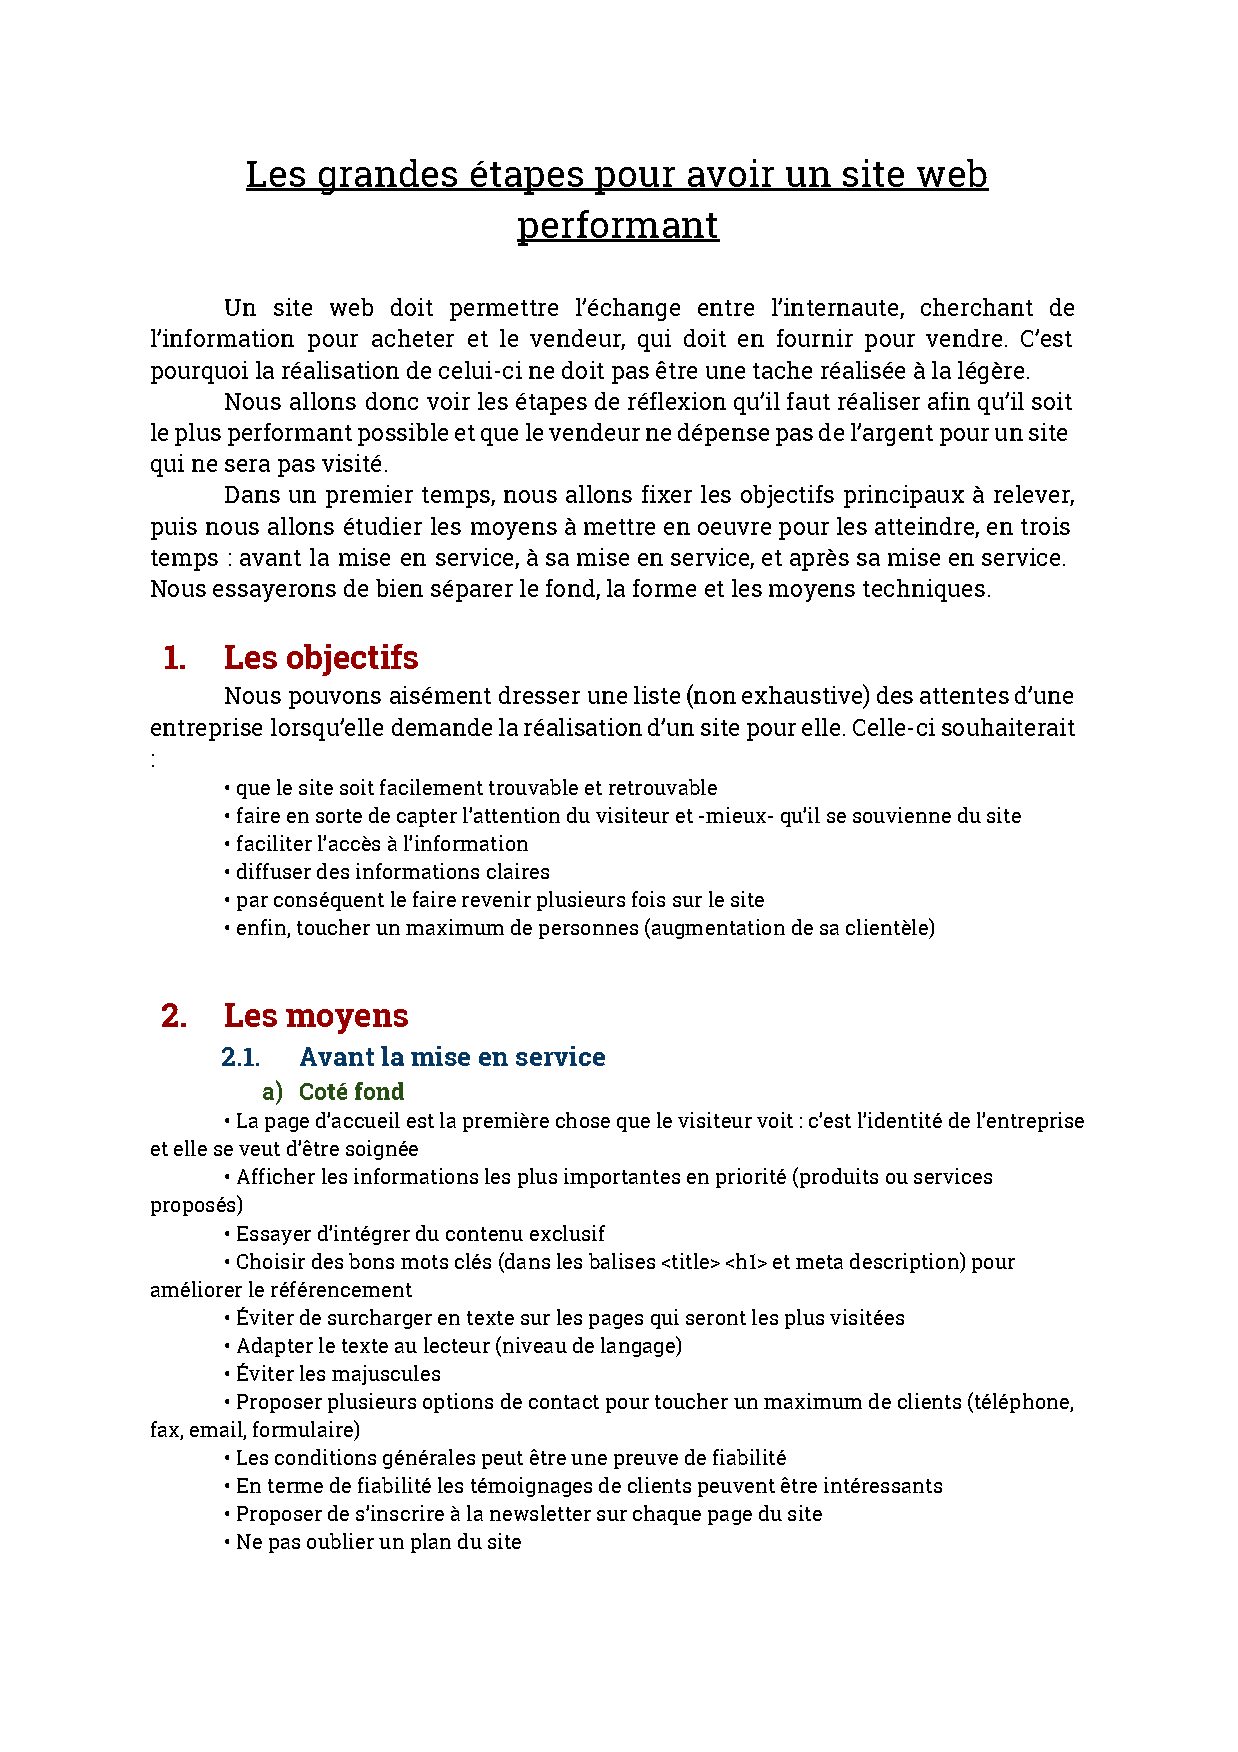
\includepdf[pages={1-2}]{pdf/Processus_site_performant.pdf}

\chapter{Annexe : Processus de vérification des sites}
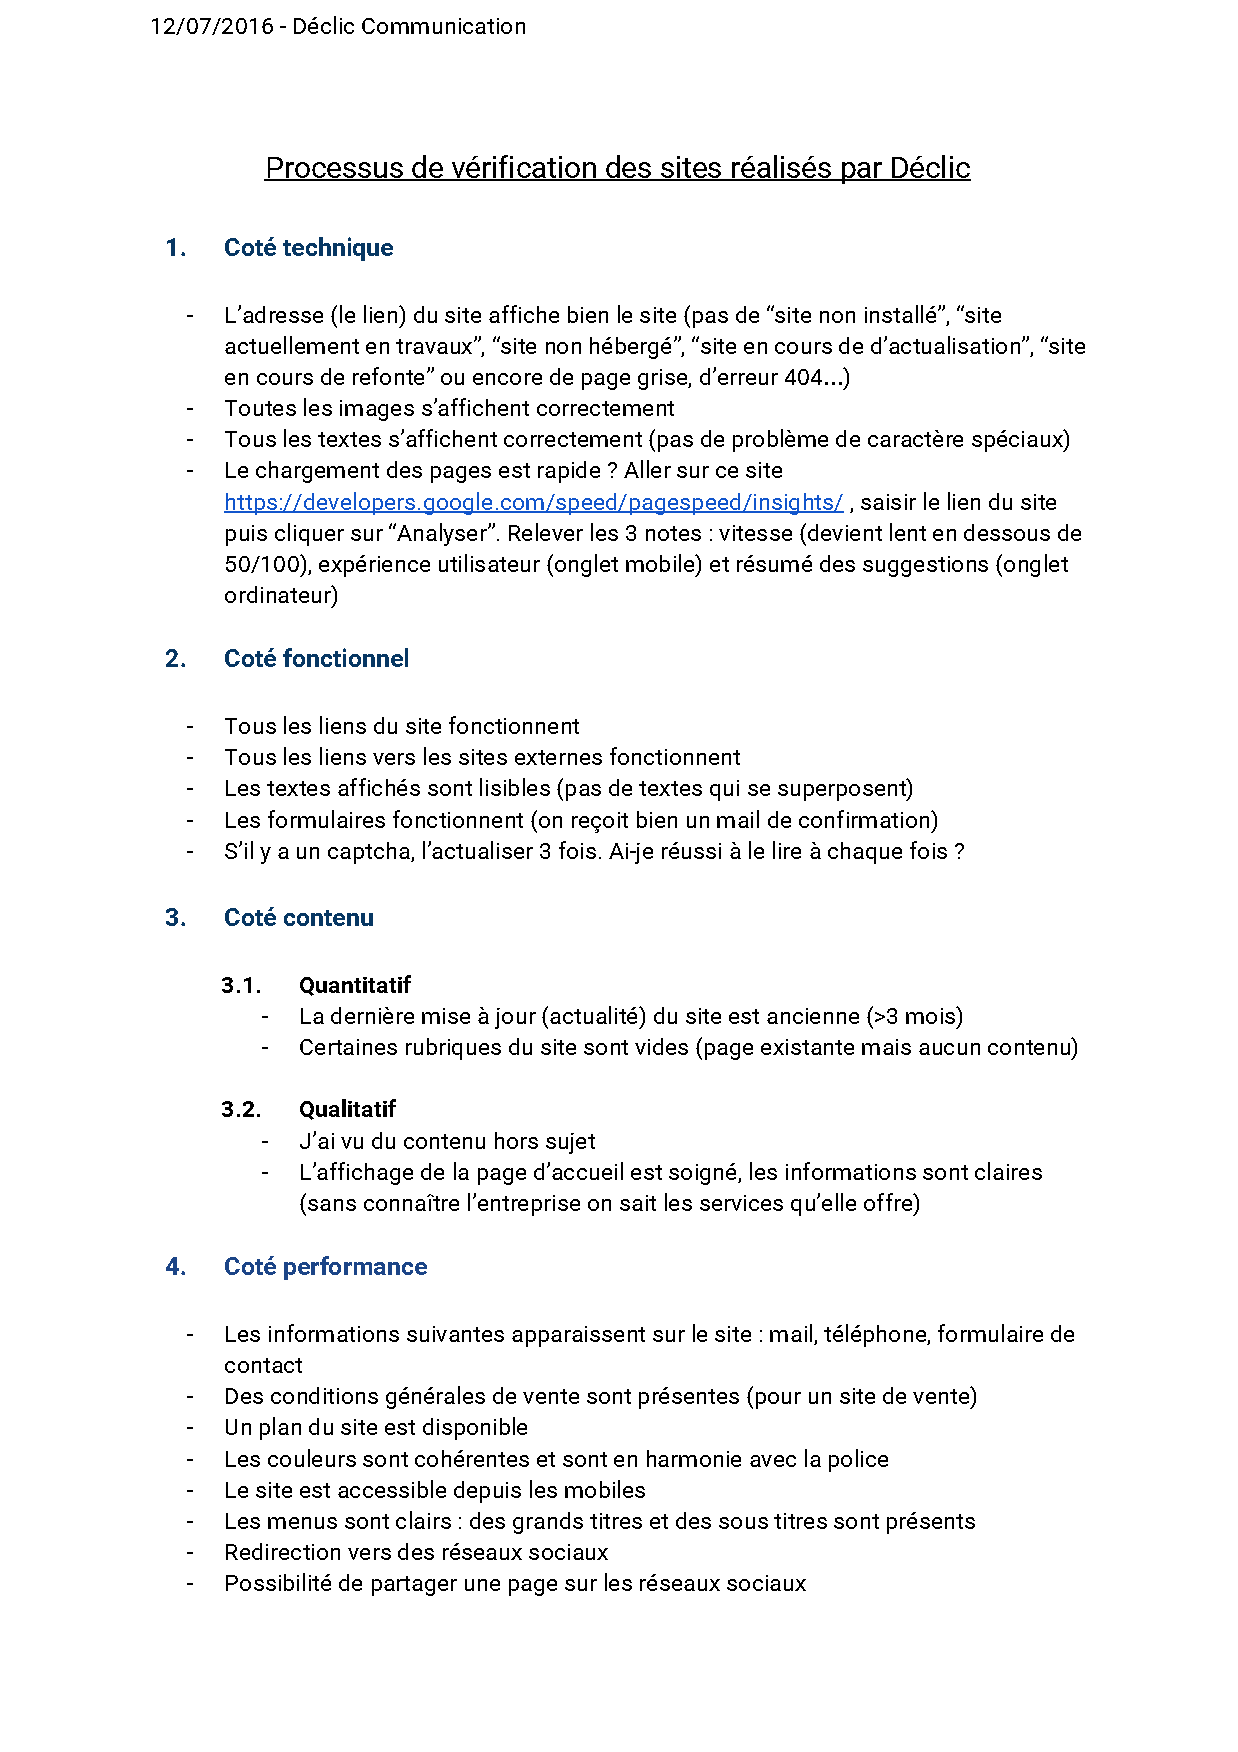
\includepdf[pages={1-2}]{pdf/Processus_de_verification_des_sites.pdf}

\chapter{Annexe : Tableaux comparatif des solutions actuelles de logiciels CRM}
\begin{figure}[h]
  \centering
  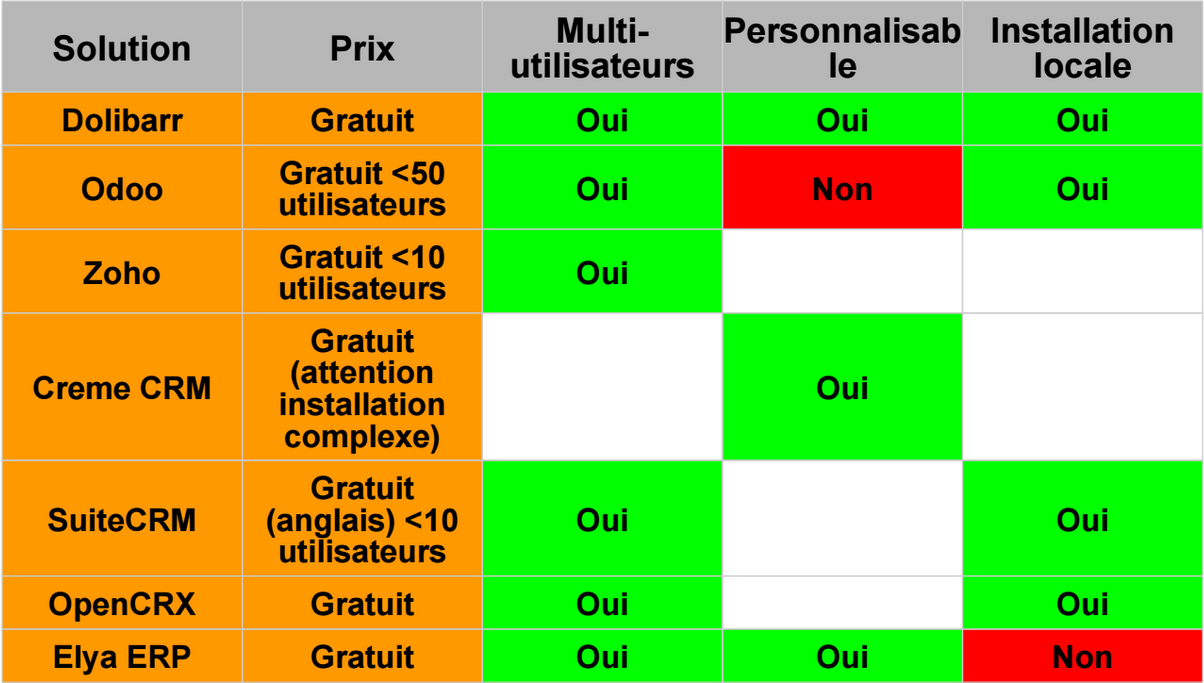
\includegraphics[width=13cm]{figures/compare1}
  \caption{Tableau comparatif 1}
  \label{fig:compare1}
\end{figure}
\begin{figure}[h]
  \centering
  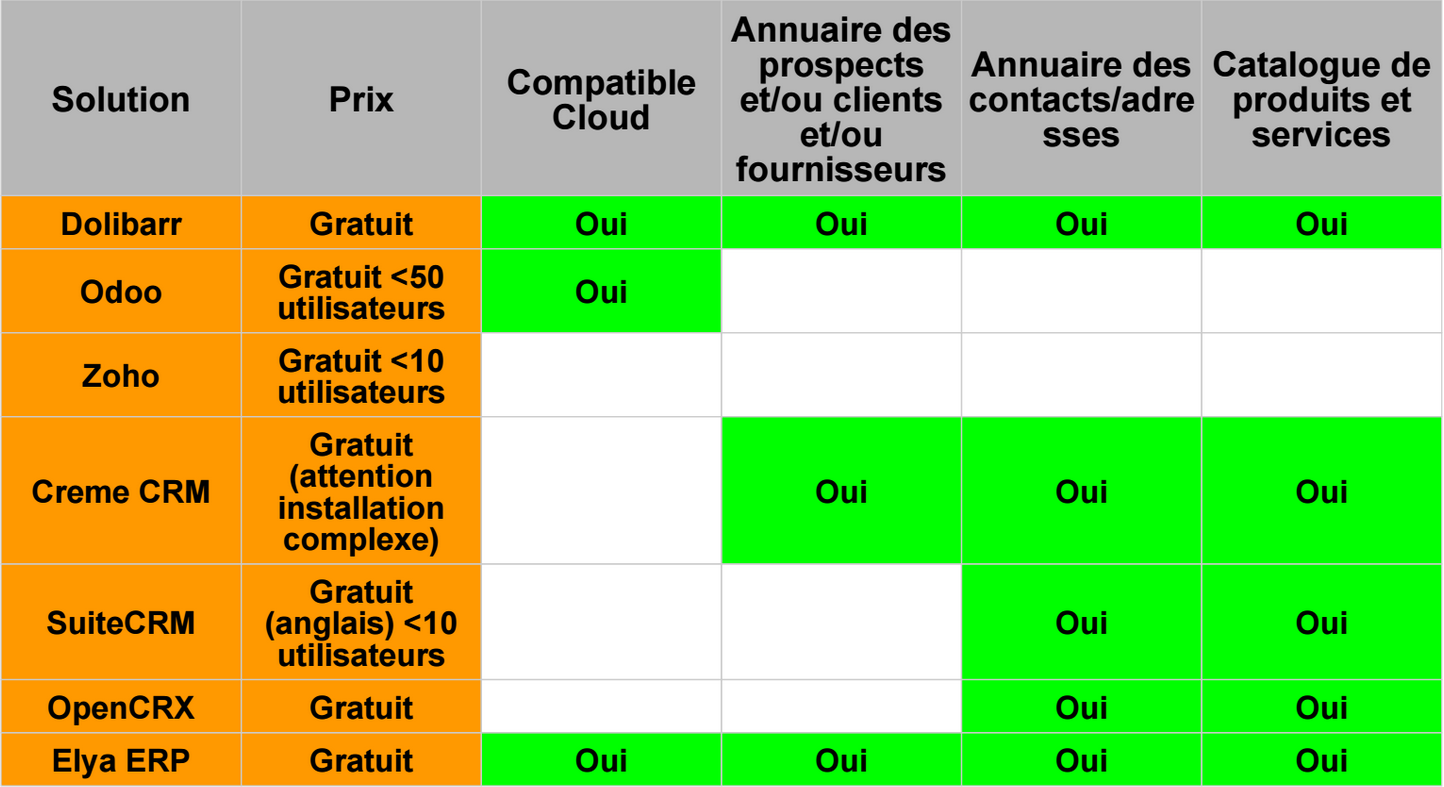
\includegraphics[width=13cm]{figures/compare2}
  \caption{Tableau comparatif 2}
  \label{fig:compare2}
\end{figure}
\begin{figure}[h]
  \centering
  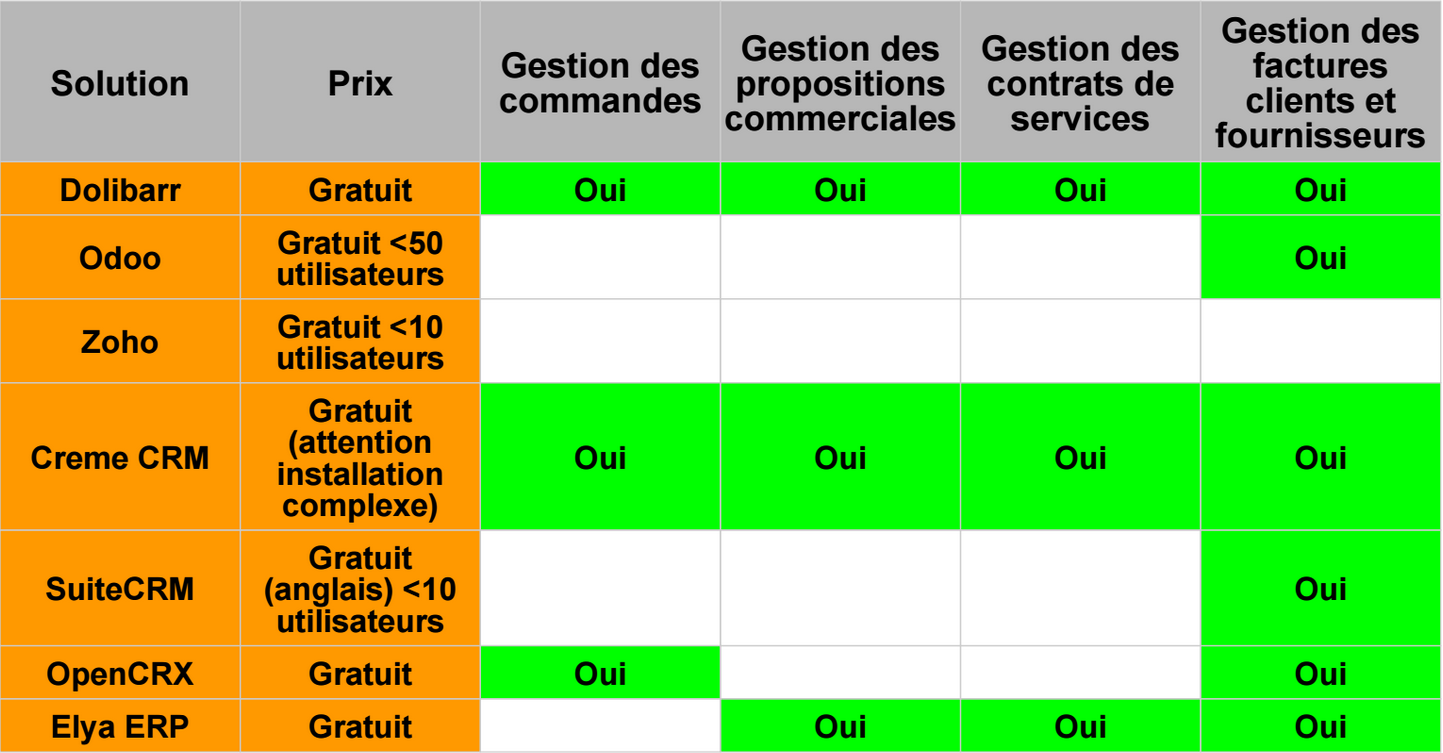
\includegraphics[width=13cm]{figures/compare3}
  \caption{Tableau comparatif 3}
  \label{fig:compare3}
\end{figure}
\begin{figure}[h]
  \centering
  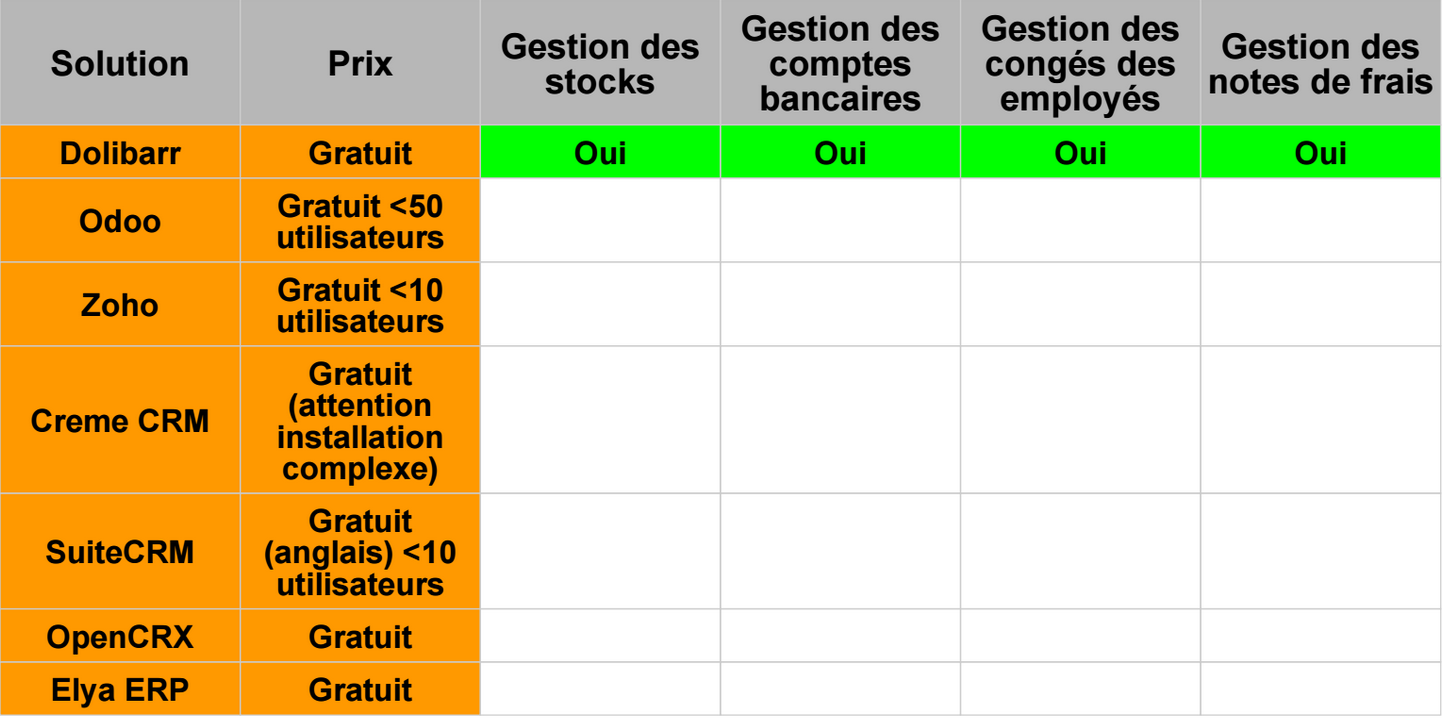
\includegraphics[width=13cm]{figures/compare4}
  \caption{Tableau comparatif 4}
  \label{fig:compare4}
\end{figure}
\begin{figure}[h]
  \centering
  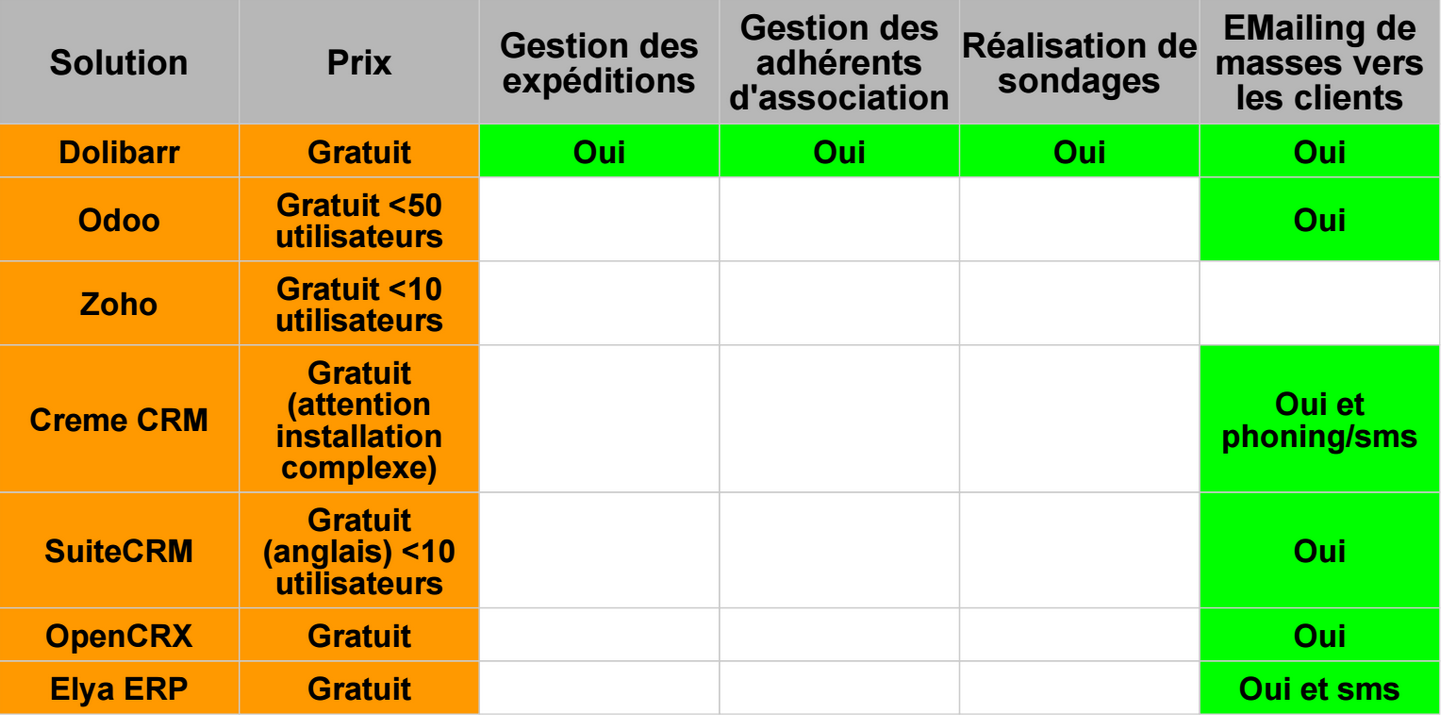
\includegraphics[width=13cm]{figures/compare5}
  \caption{Tableau comparatif 5}
  \label{fig:compare5}
\end{figure}
\begin{figure}[h]
  \centering
  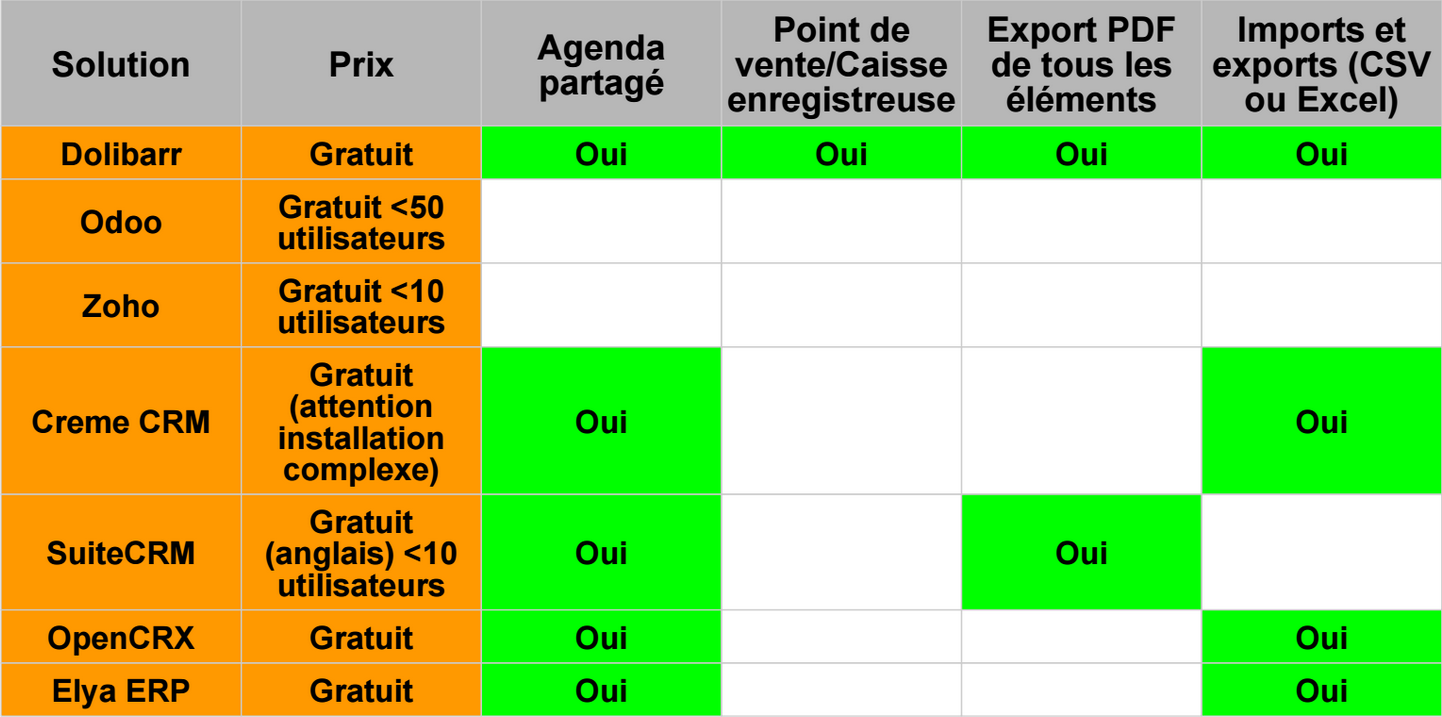
\includegraphics[width=13cm]{figures/compare6}
  \caption{Tableau comparatif 6}
  \label{fig:compare6}
\end{figure}
\begin{figure}[h]
  \centering
  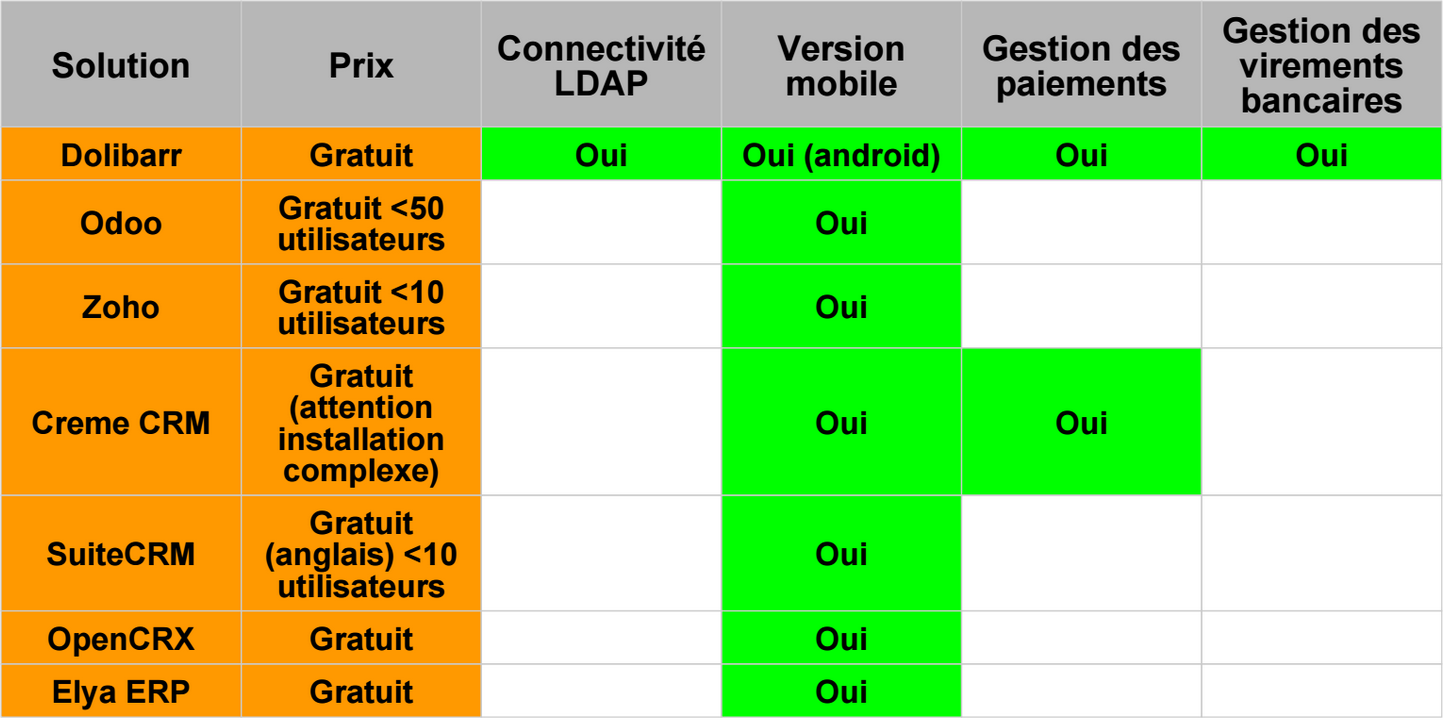
\includegraphics[width=13cm]{figures/compare7}
  \caption{Tableau comparatif 7}
  \label{fig:compare7}
\end{figure}
\begin{figure}[h]
  \centering
  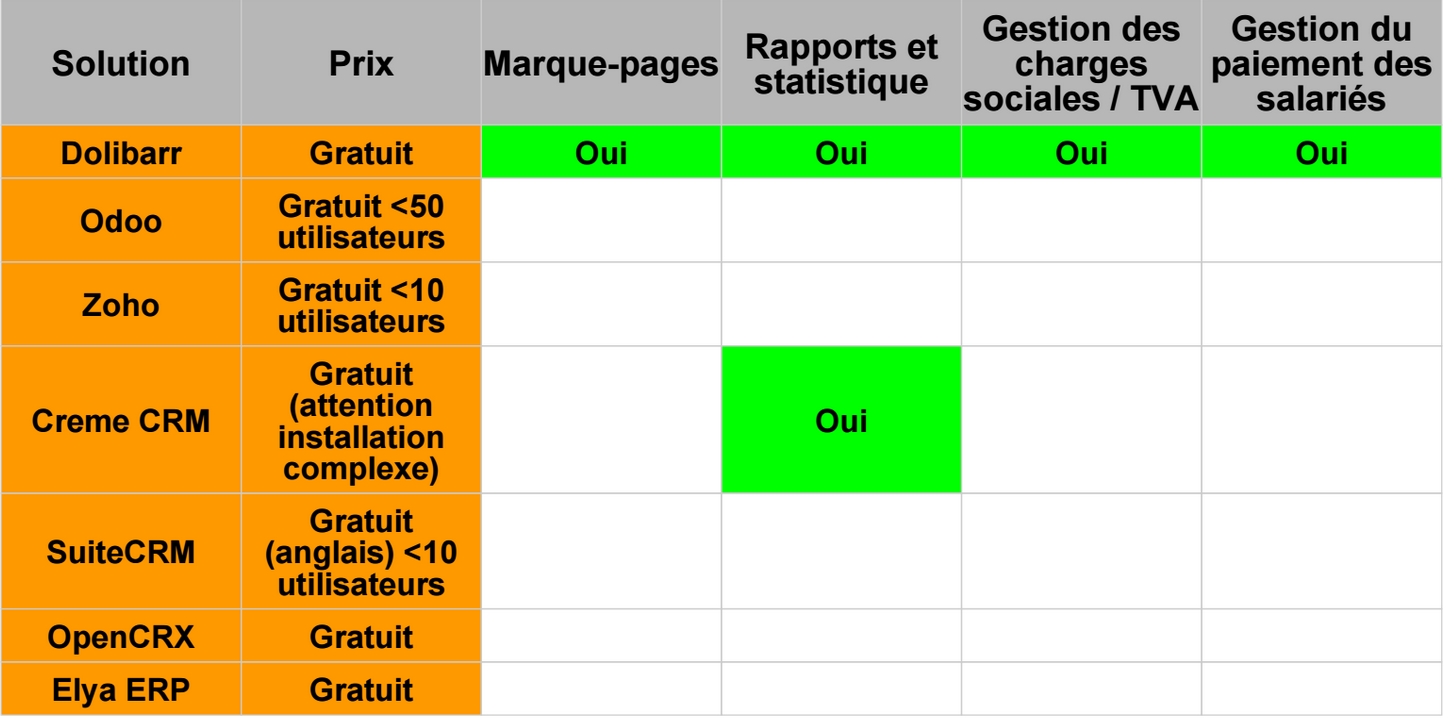
\includegraphics[width=13cm]{figures/compare8}
  \caption{Tableau comparatif 8}
  \label{fig:compare8}
\end{figure}

\chapter{Annexe : Exemples de fichiers générés avec Dolibarr}

\includepdf{pdf/commande_fournisseur.pdf}
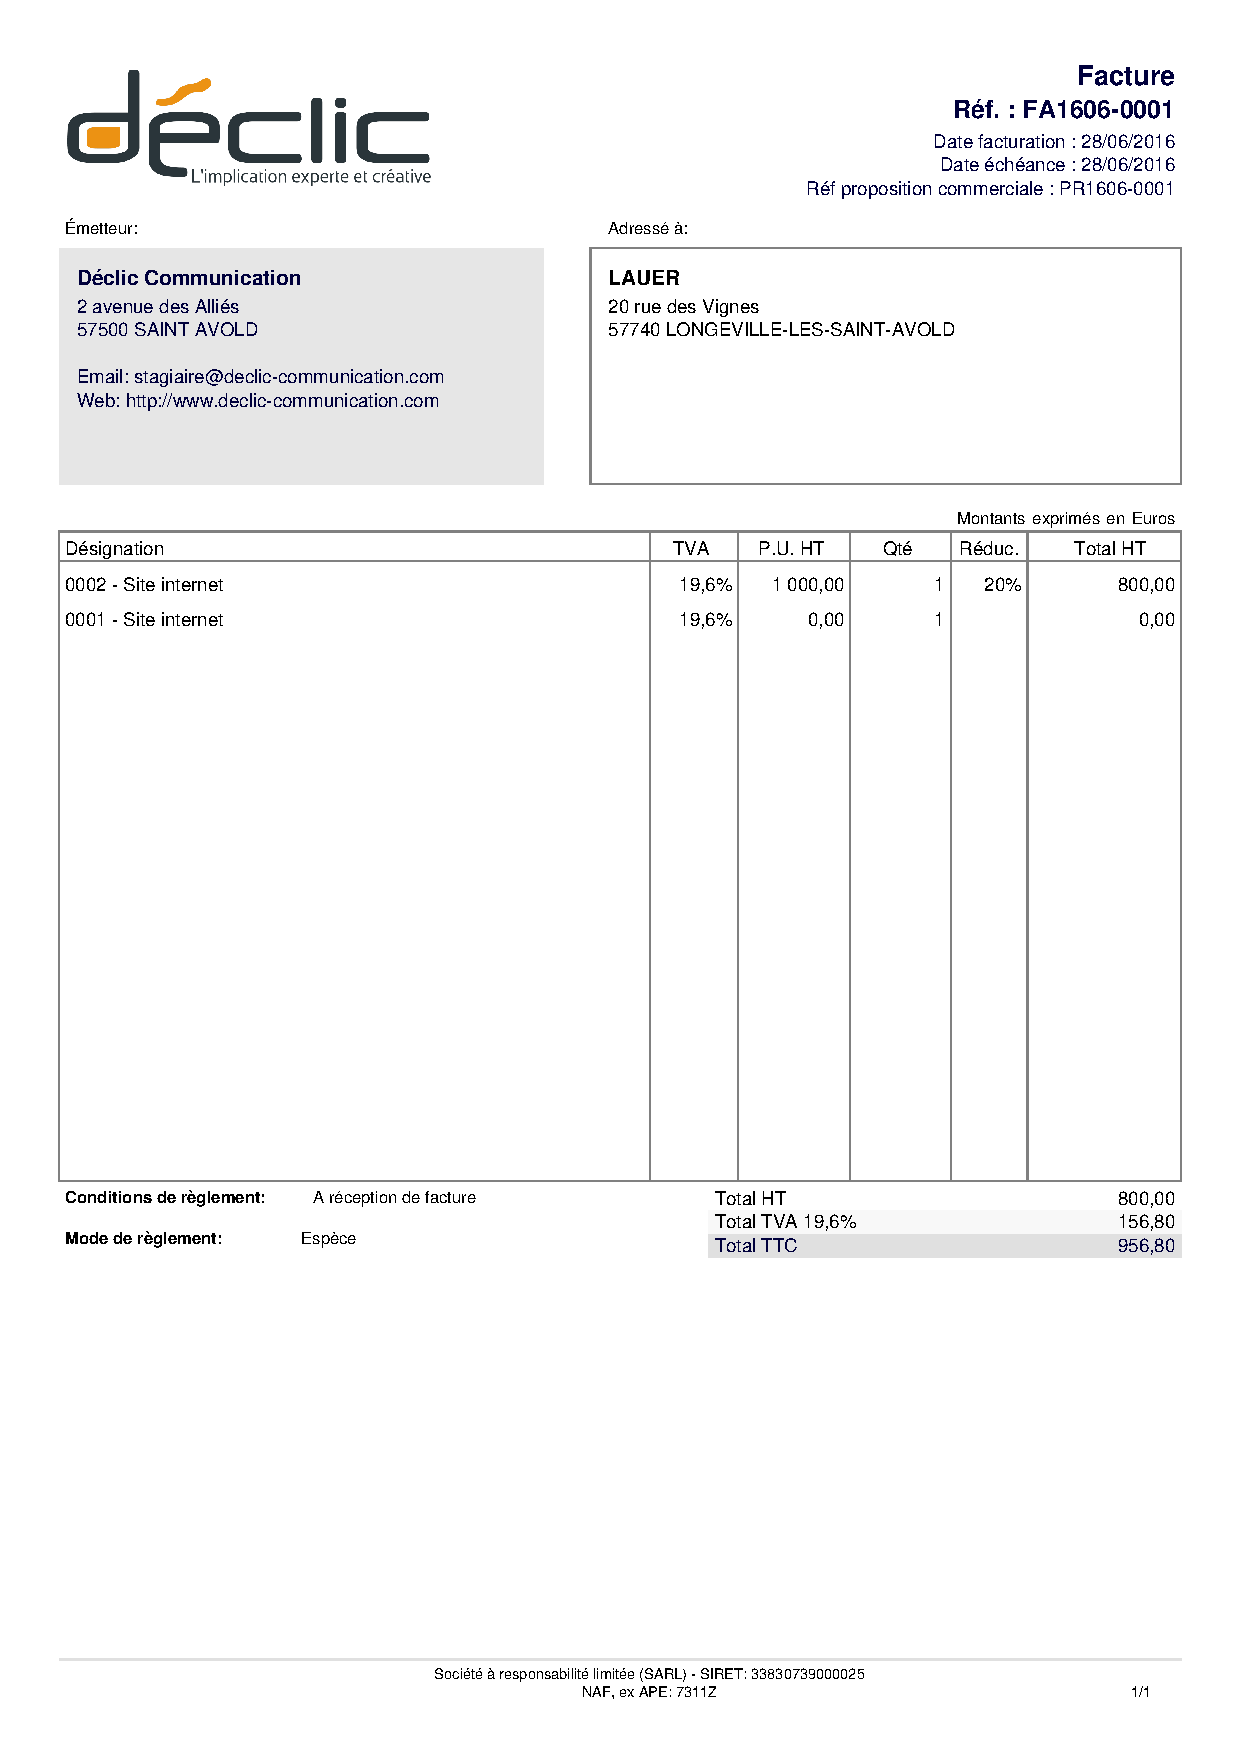
\includepdf{pdf/facture_client.pdf}
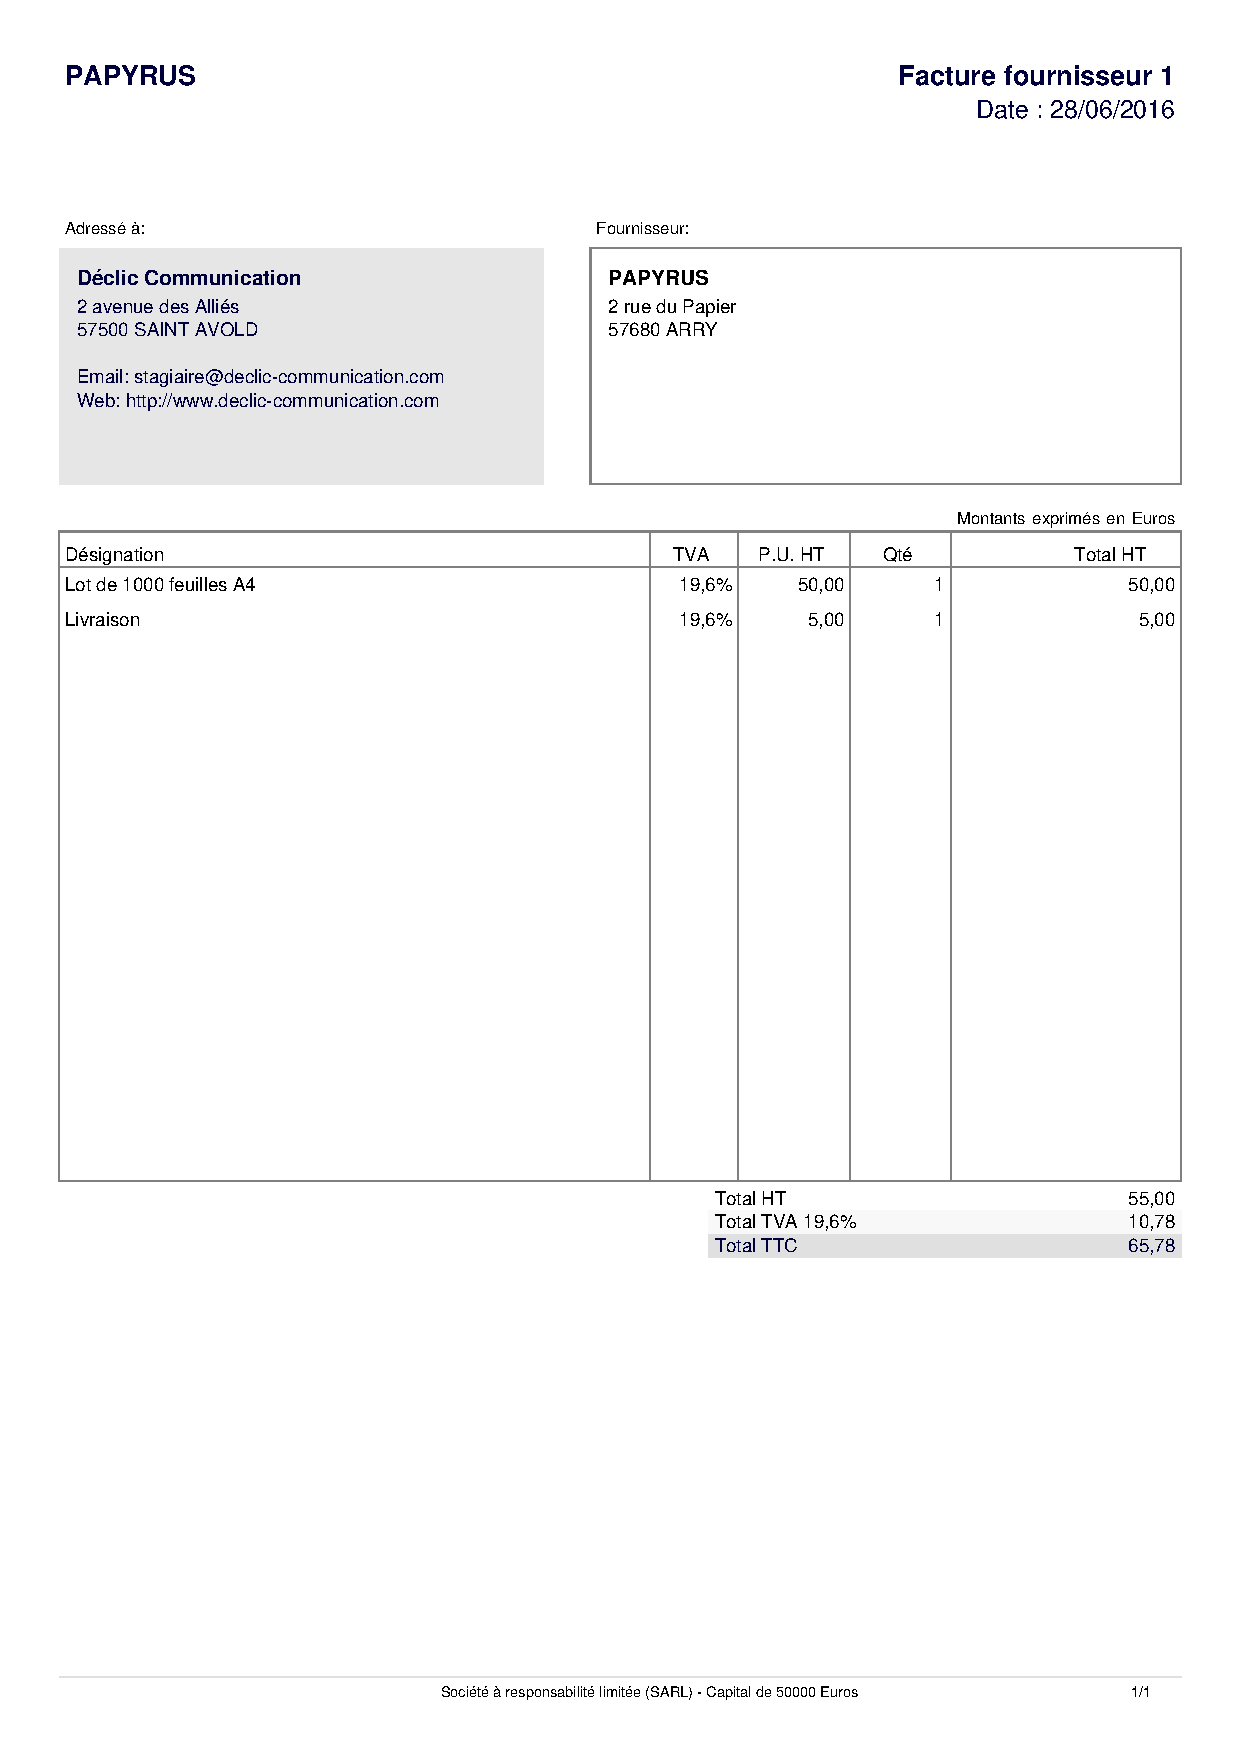
\includepdf{pdf/facture_fournisseur.pdf}

\chapter{Annexe : Equation du futur}
\begin{figure}[h]
  \centering
  
\includegraphics[width=18cm]{figures/equation_du_futur}
  \caption{Equation du futur}
  \label{fig:futurEquation}
\end{figure}



\cleardoublepage
\thispagestyle{empty}

\section*{Résumé}
\addcontentsline{toc}{chapter}{Résumé}
Ce document présente le travail que j’ai effectué lors de mon stage de 2ème année à Télécom Nancy. Il s’est déroulé dans l’entreprise Déclic Communication à Saint-Avold, en Moselle et a duré 7 semaines. Mon rapport se divise en plusieurs grandes parties, qui correspondent aux tâches principales que j’ai réalisé. Dans la dernière partie, j’expose le bilan de ce stage ainsi que les difficultés rencontrées.
Les tâches principales de mon stage ont été les projets suivants : la réalisation d’un processus de vérification des sites réalisés par l’entreprise, des recherches dans le cadre de l’automatisation de mise à jour d’une base de données Wordpress, le projet du château de Saint Sixte, une étude dans le but d’une éventuelle migration de logiciel CRM et le développement d’un email responsive design.


{\bf Mots-clés : logiciel CRM, emailing responsive design, installation réseau LAN, mise à jour de BDD Wordpress}


\section*{Abstract}
\addcontentsline{toc}{chapter}{Abstract}
This document presents the work I did during my 2nd year internship. It took place at the company Declic Communication in Saint-Avold, in Moselle and lasted 7 weeks. My report is divided in several big sections which correspond to the main tasks I realized. In the last section, I will do a review of my internship and talk about the difficulties I met. The main tasks of my internship were : the creation of a verification process for the finished websites, research in automating updates to Wordpress database, a project for the castle of Saint Sixte, a study for a potential migration of CRM software and the development of a responsive design email.

{\bf Keywords : CRM software, responsive emailing, LAN installation, updating Wordpress database}


\end{document}
